\chapter{The SPACE Analysis}
After introducing the detector workings, reconstruction and analysis techniques, background contributions and the signature of the signal, this chapter gives an overview of analysis. Starting from data processed with basic reconstructions and requirements a workflow was set up to try to discriminate events that are most likely of known physical interactions from the rare events that are sought for in this analysis. These events would originate from the theoretical particles with an anomalous charge (see Chapter \ref{ch:theoreticalmotivation}). The analysis was adopted the "SPACE" analysis, which stands for a "Search for Particle with Anomalous ChargE".

\section{Filter selection}
As explained in Section \ref{subsec:filters}, the data is processed through multiple filters. Since this analysis is the first of its kind in the collaboration, no processed dataset from other analyses was used. Filters had to be selected for proper comparison of data and Monte Carlo and I have chosen to optimize the signal to background ratio to select which filters should be included. An illustration is given in Fig. \ref{fig:filterrate}. This filter selection will be referred to as \textit{Level2b}, as a simple addition to filter processing in Level2 (see Section \ref{sec:processing}). 

\begin{figure}
\centering
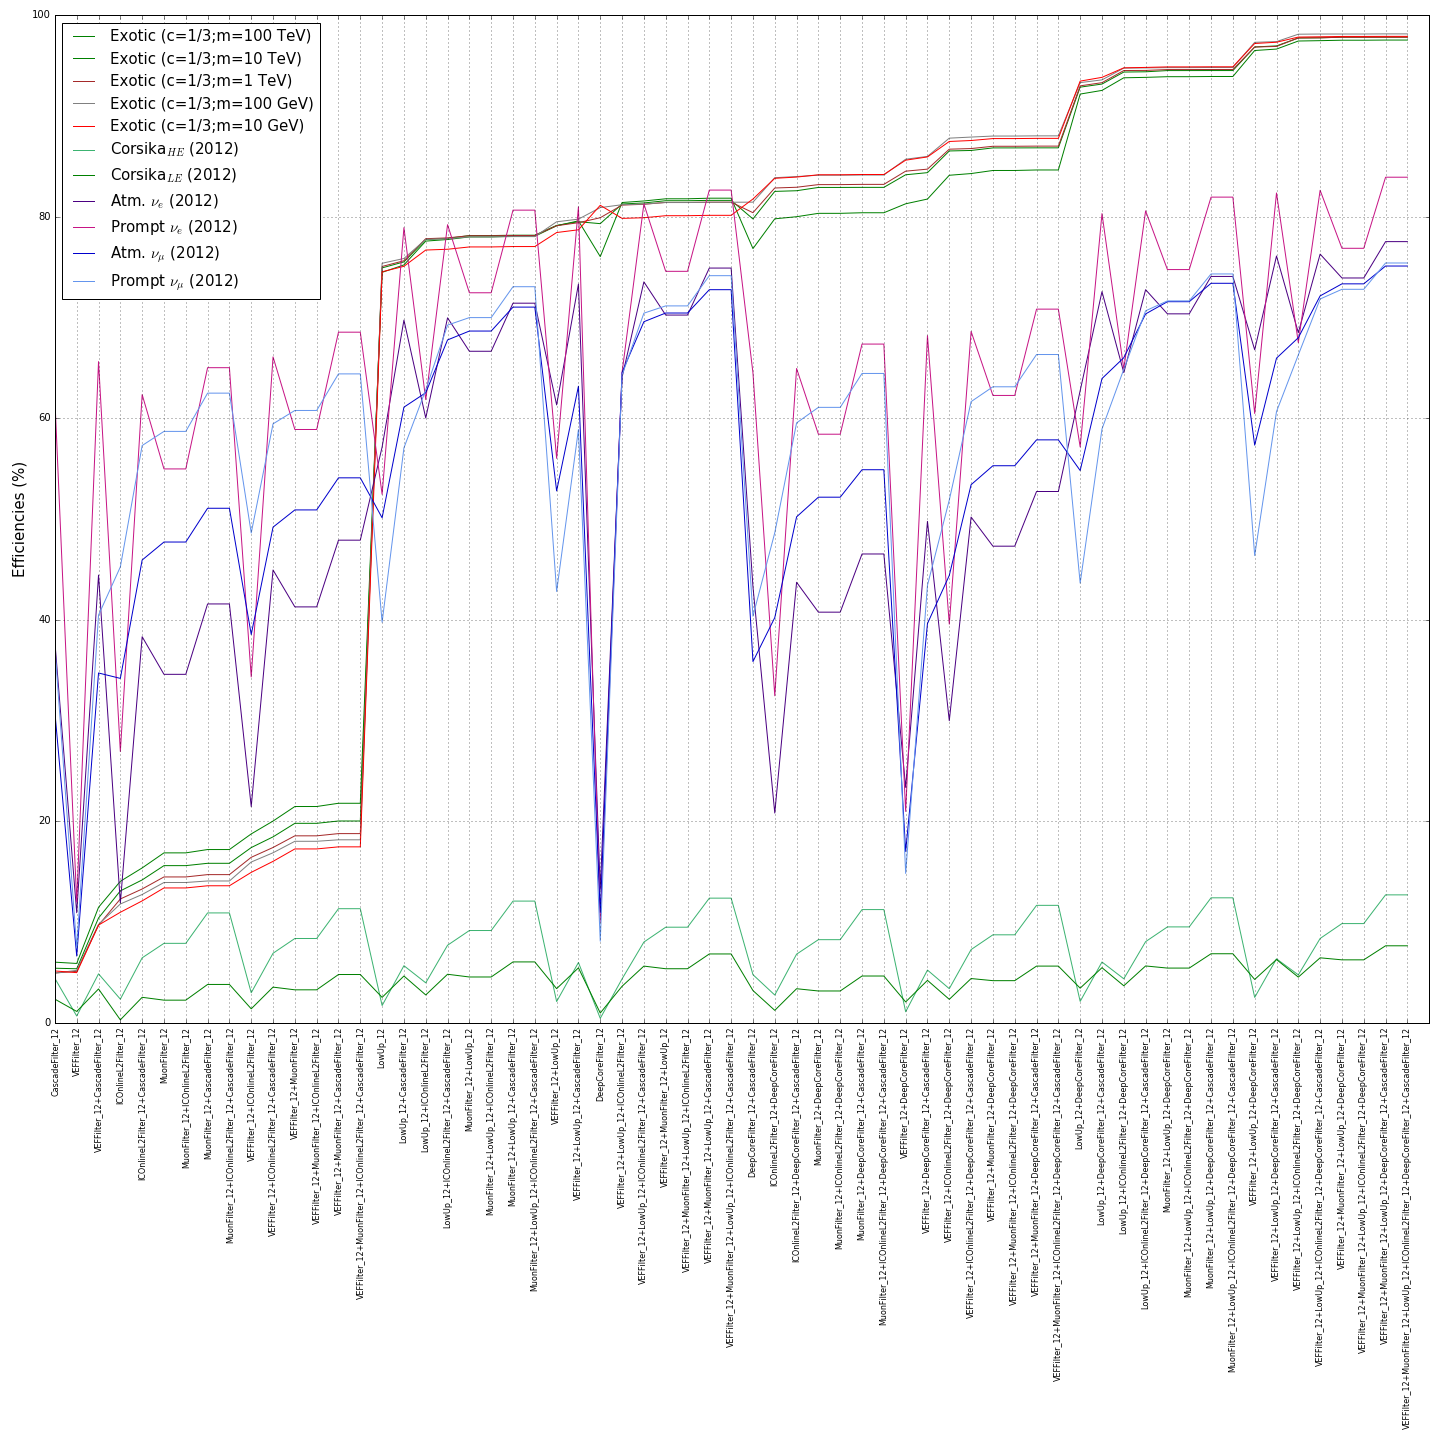
\includegraphics[width=\textwidth]{chapter8/img/FilterRate.png}
\caption{Illustration of the efficiencies of several filters and their possible combinations. The x-axis was determined by starting with filter selections that had a low efficiency in signal selection and range in function of performance. Five signal points for a fixed charge and different mass show similar results. Exotic SMPs with charges 1/2 and 2/3 show very similar results but are left out for a better visualization.}
\label{fig:filterrate}
\end{figure}

\subsection{VEF}
The Vertical Event Filter (VEF) is designed to be used for oscillation and Earth WIMP analyses and makes use of the string trigger (see Section \ref{subsec:triggers}). An SMP that travel alongside a string, or closeby, can trigger optical modules while the total light yield of an event is low, making this filter an ideal addition to the filters that are selected. In addition, the filter removes HLC hits in the top 5 DOM layers to reduce the muonic component from air shower events. Other selection cuts, try to optimize the search efficiency for WIMP events in particular. For example, the LF zenith angle should be higher than 68.7$^\circ$. More information can be found in Ref. \cite{VEF2012}.

%meeste hiervan: https://docushare.icecube.wisc.edu/dsweb/Get/Document-62750/VEF_2013_proposal.pdf

\subsection{LowUp}
The LowUp filter is again mainly designed for WIMP searches, but also atmospheric neutrino analysis and is mainly designed to capture up-going muons with an energy below 1 TeV. The majority of the events that are selected by this filter make use of the in-ice Volume Trigger (see Table \ref{tab:trigger}), but also the in-ice SMT8, in-ice String and SMT3-DeepCore triggers are run over for completeness. The selection cuts are loose selections required to look for up-going track-like particles. For example, the zenith angle of the reconstructed particle should have an angle of 80$^\circ$ or higher and the difference between the maximal z-coordinate and minimal z-coordinate of hit DOMs should be less than or equal to 600 m. More information can be found in Ref. \cite{LowUp2012}.

%je hebt een Nchan>=5 cut in je L4 zodat veranderingen in LowUp niet uitmaken :-)

\subsection{Online Muon L2}
The Online Muon L2 filter is a subset of the Muon Filter (see Ref. \ref{Muon2012}) and tries to select the most interesting muon-like events while reducing the rate of the filter from around 30 Hz to 5 Hz, reducing the data with a factor of 6. Historically this subset was processed data from the Muon Filter, but after realizing that this could be done online and because many analyses made use of this selection, it was chosen to implement it as a separate filter. The filter tries to select both up-going and down-going muons, with different selection cuts depending on the zenith angle of the particle reconstruction. The four selection ranges are defined as:
\vspace{2mm}
\begin{itemize}
\item $180^\circ \geq \theta_\textrm{MPE} \geq 115^\circ$
\item $115^\circ > \theta_\textrm{MPE} \geq 82^\circ$
\item $82^\circ > \theta_\textrm{MPE} \geq 66^\circ$
\item $66^\circ > \theta_\textrm{MPE} \geq 0^\circ$
\end{itemize}
where the particle reconstruction was done with MPE (Section \ref{subsec:spempe}), which was feasible if it only had to be done on the events passing the Muon Filter. The first two regions have an efficiency\footnote{Here defined as having a reconstruction within 3$^\circ$ of the MC truth.} higher than 99\%. The down-going region require more stringent cuts to remove the less interesting muons from air showers. The variables used are the number ot hit DOMs, likelihood parameters, number of PEs and so on. More information can be found in Ref. \cite{OnlineMuonL22012}.

\textcolor{red}{Verhoogt uw signaal niet zo veel omdat je enkel upgoing signaal gebruikte om dit te testen.}

\subsection{DeepCore}
Additionally a DeepCore specialized filter was added to account for SMP tracks that partially traverse the more densly instrumented DC detector. Due to the low amount of light produced by these dim tracks, adding the DeepCore filter that is specialized for this part of the detector proved to be of significant importance.

The DeepCore filter was designed to look for very dim events coming from, e.g., dark matter, low-energy neutrino oscillations, and studies in observing atmospheric neutrinos below 100 GeV. The fiducial volume used for this filter consists of
\vspace{2mm}
\begin{itemize}
\item the bottom 22 DOMs on the IceCube strings 25, 26, 27, 34, 35, 36, 37, 44, 45, 46, 47 and 54;
\item the bottom 50 DOMs on the DeepCore strings 79-86.
\end{itemize}
\vspace{2mm}
These strings are indicated in Fig. \ref{fig:deepcorestrings}.\\

\begin{figure}[t]
\centering
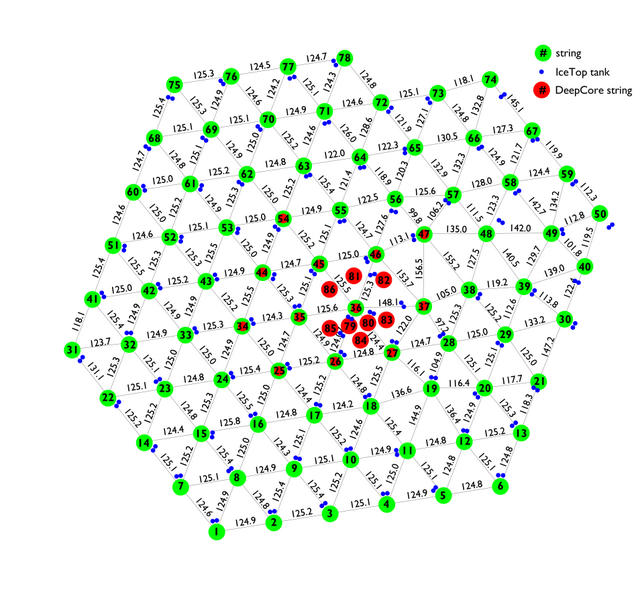
\includegraphics[width=0.55\textwidth]{chapter8/img/stringview.jpg}
\caption{Aerial view of the IceCube strings (and IceTop tanks) where the DeepCore fiducial volume is defined by the DeepCore strings (red) and several surrounding in-ice IceCube strings (green and red).}
\label{fig:deepcorestrings}
\end{figure}

\noindent The filter uses the DeepCore SMT3 trigger and calculates the COG position. Two layers are used as a veto to remove events that probably originate from atmospheric muons. More information can be found in Ref. \cite{DeepCore2012}.

\subsection{Burnsample checks}
Before further processing, the burn sample (Section \ref{sec:burnsample}) is compared over the different years that are used in the analysis. This is shown in Figure \ref{fig:burnsamplechecks}. More information on the burn sample can be found in Section \ref{sec:burnsample}.

\begin{figure}[t]
\centering
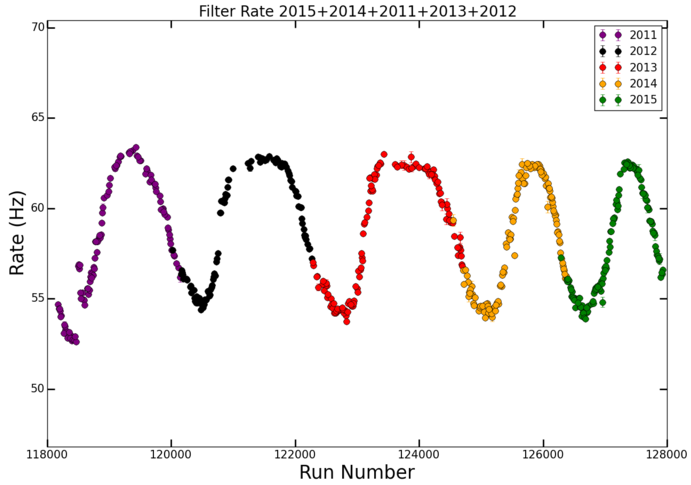
\includegraphics[width=0.49\textwidth]{chapter8/img/FilterRatePerRun.png}
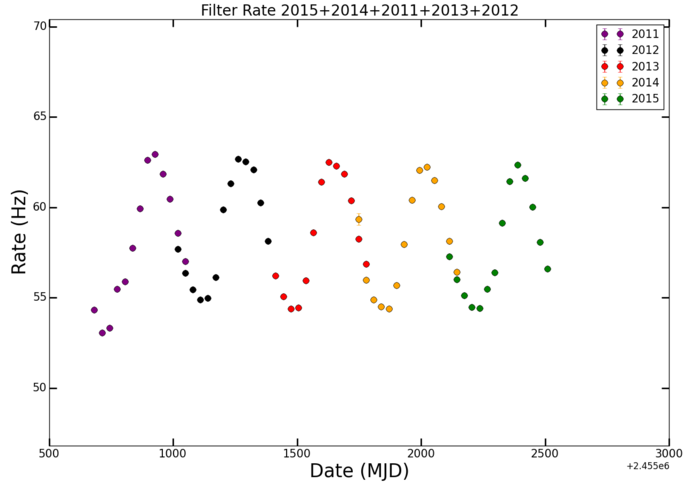
\includegraphics[width=0.49\textwidth]{chapter8/img/FilterRatePerMonth.png}
\caption{\textit{Left: }Total rate of the combined filters in function of the run number. The sine wave pattern from seasonal variations in the atmosphere (see Section \ref{subsub:corsika}) is clearly visible and consisten throughout the years. The x-axis is more spread out in the first years as there were more test runs. The shift in data rate in early 2011 runs is due to the DOM software change that was introduced in the Summer of 2011 \cite{2011rate}. This phenomenon is well understood and since the changes are minimal it was chosen to keep these runs. \textit{Right: }Total filter rate averaged per month. There is an overlap for each year because a new season doesn't necessarily start in the beginning of a month.}
\label{fig:burnsamplechecks}
\end{figure}

\section{Level 3}
The combined filter selection leads to a total rate of $\sim60$ Hz, or $\sim1.9$ billion events per year. The average event size at Level2 is around 15 kB, which would result into around 30 TB of data per year.

Therefore, five quality cuts are implemented with a goal that is threefold:
\vspace{2mm}
\begin{enumerate}
\item reduce the total rate of the data,
\item improve the signal to background ratio, getting rid of uninteresting events,
\item improve the agreement between data and Monte Carlo.
\end{enumerate}
\vspace{2mm}
\noindent These cuts are shown in Figs. \ref{fig:level3cuts1}, \ref{fig:level3cuts2} and \ref{fig:level3cuts3}.

\subsection{Zenith angle cut}
Even though there are no up-going muons from air showers expected, the vast majority of events that pass the filter selection remain from misreconstructed muons. Even though there is only a small chance of these events to have a large misreconstructed zenith angle. The expected flux of air showers is so much larger compared to the assumed signal flux to such an extent that is dominates with orders of magnitude. The majority still has an reconstructed zenith angle lower than 90$^\circ$. Therefore the zenith angle cut was set at an angle of 

\begin{equation}
\theta_\textrm{zen} (\textrm{MPE}) \geq 85^\circ.
\end{equation}

\begin{figure}[ht]
\centering
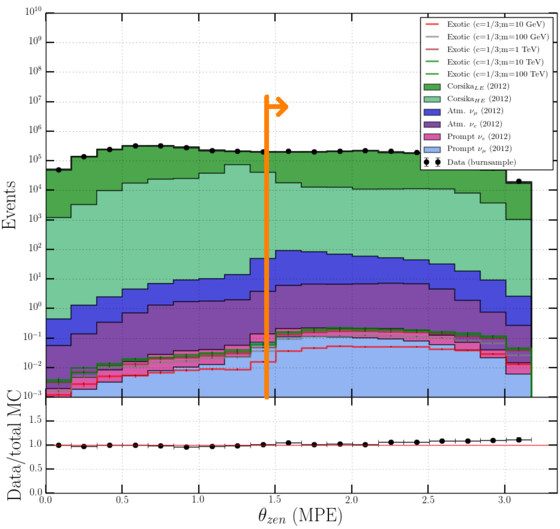
\includegraphics[width=0.49\textwidth]{chapter8/img/1D_stack_mpefit_zenith.png}
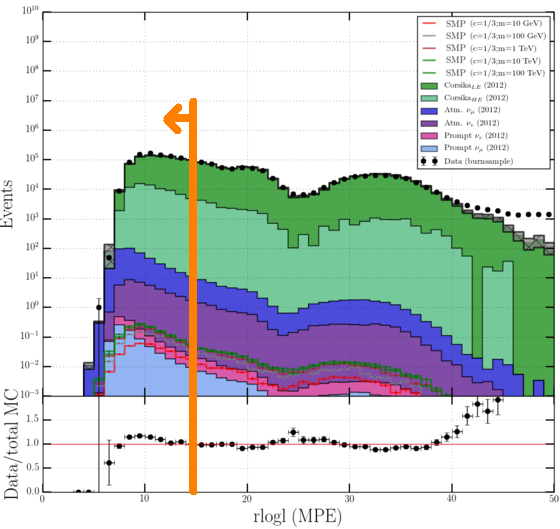
\includegraphics[width=0.49\textwidth]{chapter8/img/1D_stack_mpefit_rlogl.png}
\caption{\textit{Left: }Number of events in function of MPE reconstructed zenith angle normalized to the burn sample. The upwards trend to higher zenith angles is due to the filter selections that depend on the angle. \textit{Right: }Number of events in function of rlogL normalized to the burn sample. The cuts are illustrated with an orange line, the arrow points towards the events that are kept.}
\label{fig:level3cuts1}
\end{figure}

\begin{figure}[ht]
\centering
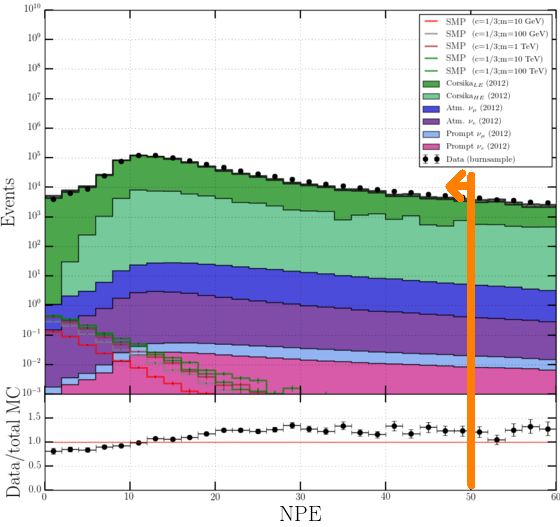
\includegraphics[width=0.49\textwidth]{chapter8/img/L3_zenithcut_gr_1p4835298642_rloglcut_less_15_1D_stack_npe.png}
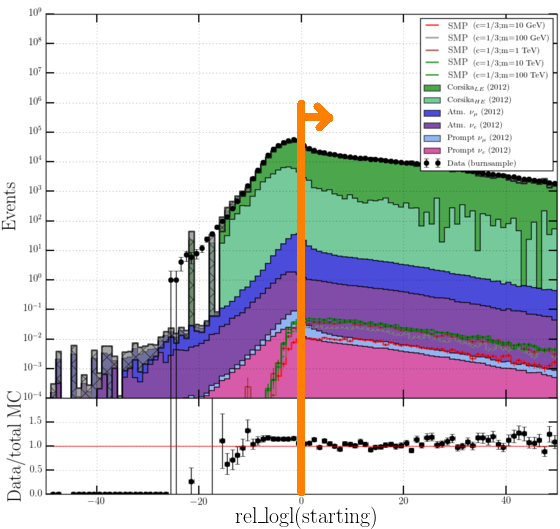
\includegraphics[width=0.49\textwidth]{chapter8/img/L3_zenithcut_gr_1p4835298642_rloglcut_less_15_npecut_less_50_1D_stack_finitereco_rllh_starting.png}
\caption{\textit{Left: }Number of events in function of number of photoelectrons (NPE) seen in the detector. \textit{Right: }Number of events in function of the starting likelihood. The cuts are illustrated with an orange line, the arrow points towards the events that are kept.}
\label{fig:level3cuts2}
\end{figure}

\begin{figure}[ht]
\centering
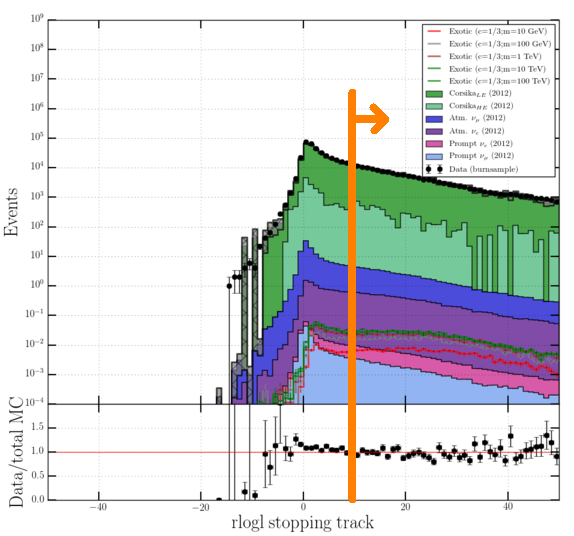
\includegraphics[width=0.49\textwidth]{chapter8/img/L3_zenithcut_gr_1p4835298642_rloglcut_less_15_npecut_less_50_startingtrackcut_hs_gr_0_1D_stack_finitereco_rllh_stopping.png}
\caption{Number of events in function of the stopping likelihood. The cut is illustrated with an orange line, the arrow points towards the events that are kept.}
\label{fig:level3cuts3}
\end{figure}

\subsection{RlogL cut}
The reduced log-likelihood, rlogL of the track reconstruction fit is used as a goodness-of-fit variable. The term ``reduced'' is used because the logarithm of the likelihood is normalized by the number of degrees of freedom (NDOF) in the track fit

\begin{equation}
\textrm{rlogL} = \frac{\log \mathcal{L}}{\textrm{NDOF}} = \frac{\log \mathcal{L}}{\textrm{NCh} - \textrm{NPara}},
\end{equation}
where NCh is the number of channels/DOMs and NPara the number of fitted parameters (3 for the position and 2 for the track). For Gaussian probability distributions this expression corresponds to the reduced chi-square. Lower values indicate better reconstructions, therefore the rlogL cut was set at a value of 

\begin{equation}
\textrm{rlogL} < 15.
\end{equation}

\subsection{NPE cut}
The number of photoelectrons seen in the detector has a clear correlation to the number of photons that were emitted from the track. From Eq. \ref{eq:franktamm} it is clear that particles with a charge $< 1$ will produce less light. Therefore a cut on the total number of photoelectrons was set at a value of 

\begin{equation}
\textrm{NPE} < 50.
\end{equation} 


\subsection{Starting rlogL cut}
The relative probability for tracks to be starting and/or stopping can be computed with FiniteReco (see Section \ref{subsec:finitereco}). Because most low-energetic muons would be starting and/or stopping in the detector, these likelihoods prove to be a powerful tool in removing these events \footnote{High energetic muons will have a higher change of being throughgoing, but would produce much more light than the dim tracks that are expected for the SMPs.}. The llh is always compared to the llh of throughgoing tracks, hence the ``relative probability''. It was chosen to place the starting rlogL at a value of 

\begin{equation}
\textrm{rlogL} = \textrm{rlogL}(\textrm{starting}) - \textrm{rlogL}(\textrm{throughgoing}) > 0. 
\end{equation}

\subsection{Stopping rlogL cut}
Analogous to the previous cut, it was chosen to place the stopping rlogL at a value of
\begin{equation}
\textrm{rlogL} = \textrm{rlogL}(\textrm{stopping}) - \textrm{rlogL}(\textrm{throughgoing}) > 10. 
\end{equation}


\section{Level 4}
As can be seen in Figs. \ref{fig:level3cuts1}, \ref{fig:level3cuts2} and \ref{fig:level3cuts3}, most of the background still originates from air showers (referred to as CORSIKA). Due to the Level 3 quality cuts, the total rate was reduced from around $\sim 60$ Hz to $\sim2$ Hz, low enough for more elaborate variables to be computed and more elaborate cleaning. In Level 4 I have implemented the IceHive splitting and cleaning tools (see Section \ref{sec:icehive}) and rerun the particle reconstructions on these ``new'' events. Additional quality cuts were added to this level to ensure higher quality events. An overview is given in Table \ref{tab:level4}. Finally, new variables were constructed to use in Level 5.

\begin{table}[]
\caption{Overview of quality cuts in Level 4.}
\label{tab:level4}
\resizebox{\textwidth}{!}{%
\begin{tabular}{|
>{\columncolor[HTML]{F1A91E}}l |c|c|c|}
\hline
Variable & \cellcolor[HTML]{F1A91E}Definition & \cellcolor[HTML]{F1A91E}Cut & \cellcolor[HTML]{F1A91E}Motivation \\ \hline
nCh & Number of hit DOMs & $\geq 5$ & Allows for better reconstructions \\ \hline
nStr & Number of hit strings & $\geq 2$ & Allows for better reconstructions \\ \hline
nStr\_in & \begin{tabular}[c]{@{}c@{}}The number of hit inner strings.\\ An inner string is not located at the edge of the detector\end{tabular} & $\geq 1$ & Reduce leak-in events \\ \hline
Fitstatus MPE & Status of MPE reconstruction & Status == 'OK' & Remove bad reconstructions \\ \hline
$\theta_{HC}$ (MPE) & Zenith angle cut on HiveCleaned pulses & $\geq 85^\circ$ & \begin{tabular}[c]{@{}c@{}}Similar to cut explained in ???:\\ focus on up-going tracks\end{tabular} \\ \hline
Innerstring domination & See text inline & == True & See text inline \\ \hline
\end{tabular}%
}
\end{table}

\subsection{Cleaning and quality cuts}
\noindent IceHive provides for a thourough cleaning method, sometimes resulting into events with a very low amount of hit DOMs. However, a minimal amount of hits is required to have reasonable and trustworthy particle reconstructions. Similarly, more than one string should have a hit to allow for better reconstructions due to the sparse distribution of the strings in the detector. Because light is able to reach the edge of the detector, even if the closest approach of the particle is tens or hunderds of meters away for very bright events, is would be near impossible to distinguish bright events far from the detector to dim tracks passing close by. Therefore, it was required that at least one string not on the edge of the detector should have hit DOMs to reduce these \textit{leak-in events}.
The zenith angle cut is re-introduced on the new event that should have better reconstructions due to cleaning and finally there is a requirement for ``innerstring domination''.

\paragraph{Innerstring domination}
There persist classes of events at the boundary of the detector, which can be a problem for an upgoing track analysis. This includes event classes as:

\vspace{2mm}
\begin{itemize}
\item (Leak in) Events which are heading towards the instrumented volume, but stop right before they reach it or pass next to, but not to far from, the detector. These leak light to the detector boundaries.
\item (Boundary) Events that penetrate the detector very shallow on the boundary lines and possibly have a cascade at the endpoint. The events have rather cascade like characteristics.
\item (Corner-clippers) Events that are throughgoing on the corners of the detector that have a COG at a corner of the detector.
\item (Leak out) Events originating from a neutrino passing through almost the entire length of the detector and only have an interaction vertex right before leaving the detector. Depending on position and angle, the reverse direction of reconstruction can be of similar probability and thus a nuisance.
\end{itemize}
\vspace{2mm}

\noindent All these event classes are not well reconstructable or have a high uncertainty in the reconstruction. It is more feasible to remove these class of events to maintain a sample of well reconstructable events. This is done here by the requirement of innerstring domination.

DOMs are defined as outer DOMs if they are one of the following:

\vspace{2mm}
\begin{itemize}
\item part of a string on edge of the detector,
\item on the bottom of strings 1-78,
\item on the top of strings 1-78.
\end{itemize}
\vspace{2mm}

\noindent The innerstring domination is set to \texttt{True} when 

\begin{equation}
\frac{\# \textrm{outer DOMs}}{\#\textrm{inner DOMs}} < 0.5.
\end{equation}

\subsection{Variable construction}
To distinguish signal from background events, variables that show a clear distribution difference prove to have the most discriminative power. In this part of the analysis, multiple new variables are introduced with this goal. Some variables used in Level 5 are already explained in the text and need no further introduction, they are shown in Fig. \ref{fig:remainingvariables}. A summary is given in Table \ref{tab:allvariables}.

\subsubsection{Commonvariables}
\label{subsub:commonvariables}
Variables that were often used in analyses often had subtle differences between them, making them prone to be a cause of errors. Multiple variable were therefore combined into one project, called ``Commonvariables''. The variables used here can be subdivided into three categories: track characteristics, hit statistics and time characteristics and are summarized in Table \ref{tab:commonvariables}. Their distributions are shown in Figs. \ref{fig:commonvariables1}, \ref{fig:commonvariables2}, \ref{fig:commonvariables3} and \ref{fig:commonvariables4}.

\begin{table}[]
\centering
\caption{List of Commonvariables used in this analysis.} 
%\vspace{2mm}
\begin{flushleft}
\begin{footnotesize}
$^\dagger$ Whenever one of the track characteristics variables is shown/mentioned, the suffix (e.g. \_50) refers to the track cylinder that was used around the track.
\end{footnotesize}
\end{flushleft}
\label{tab:commonvariables}
\resizebox{\textwidth}{!}{%
\begin{tabular}{|
>{\columncolor[HTML]{F1A91E}}l |c|c|}
\hline
Category & \cellcolor[HTML]{F1A91E}Variable & \cellcolor[HTML]{F1A91E}Description \\ \hline
\begin{tabular}[c]{@{}l@{}}Track\\ Characteristics$^\dagger$\end{tabular} & AvgDistToDom & \begin{tabular}[c]{@{}c@{}}The average distance of the DOMs to the reconstructed track, \\ weighted by the total charge of each DOM.\end{tabular} \\ \cline{2-3} 
 & EmptyHits & \begin{tabular}[c]{@{}c@{}}The maximal track length along the reconstructed track that \\ got no hits within a cylinder around the track.\end{tabular} \\ \cline{2-3} 
 & TrackSeparation & \begin{tabular}[c]{@{}c@{}}Distance how far the COG positions of the first and the \\ last quartile of the hits are separated from each other.\end{tabular} \\ \cline{2-3} 
 & TrackDistribution & \begin{tabular}[c]{@{}c@{}}The track hits distribution smoothness value {[}-1;1{]} \\ shows how smooth the hits of the given pulse series\\ within the specified track cylinder radius are distributed \\ along the track.\end{tabular} \\ \hline
Hit Statistics & ZTravel & \begin{tabular}[c]{@{}c@{}}Z value of first quartile (in time) of the hit DOMs is calculated.\\ ZTravel is the average difference of the z value of all hit DOMs\\ with the first quartile z value.\end{tabular} \\ \cline{2-3} 
 & ZMax & The maximum z of all hit DOMs. \\ \hline
\begin{tabular}[c]{@{}l@{}}Time\\ Characteristics\end{tabular} & ZPattern & \begin{tabular}[c]{@{}c@{}}All first pulses per DOM are ordered in time. If a DOM\\ position of a pulse is higher than the previous ZPattern\\ is increased with +1. If the second pulse is located lower \\ in the detector ZPattern decreases with -1. \\ In general this variable gives a tendency of the direction of a track.\end{tabular} \\ \hline
\end{tabular}%
}
\end{table}

\begin{figure}
\centering
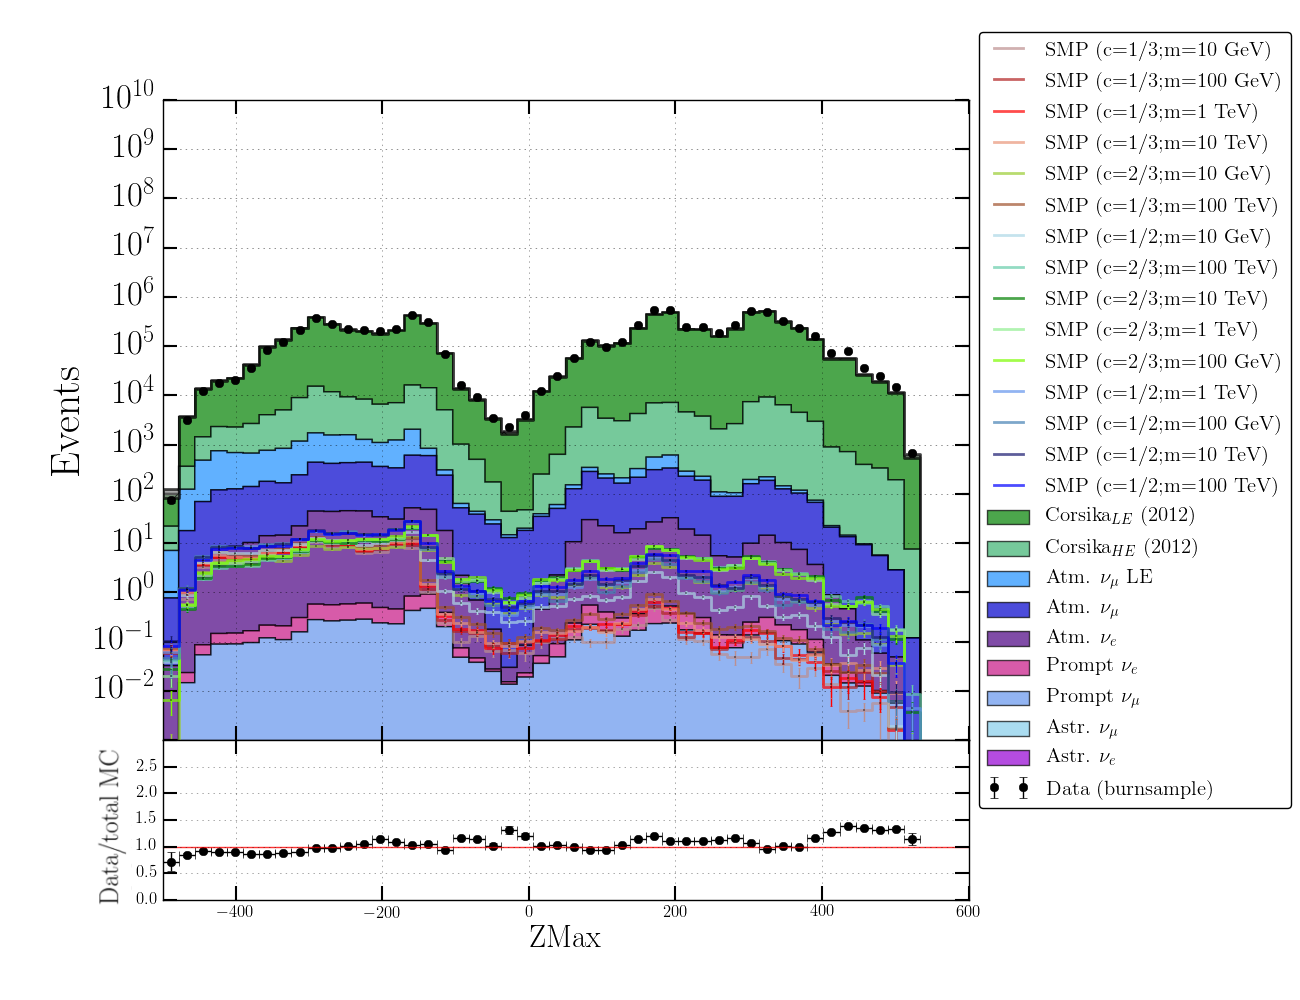
\includegraphics[width = 0.49\textwidth]{chapter8/img/1D_stack_zmax.png}
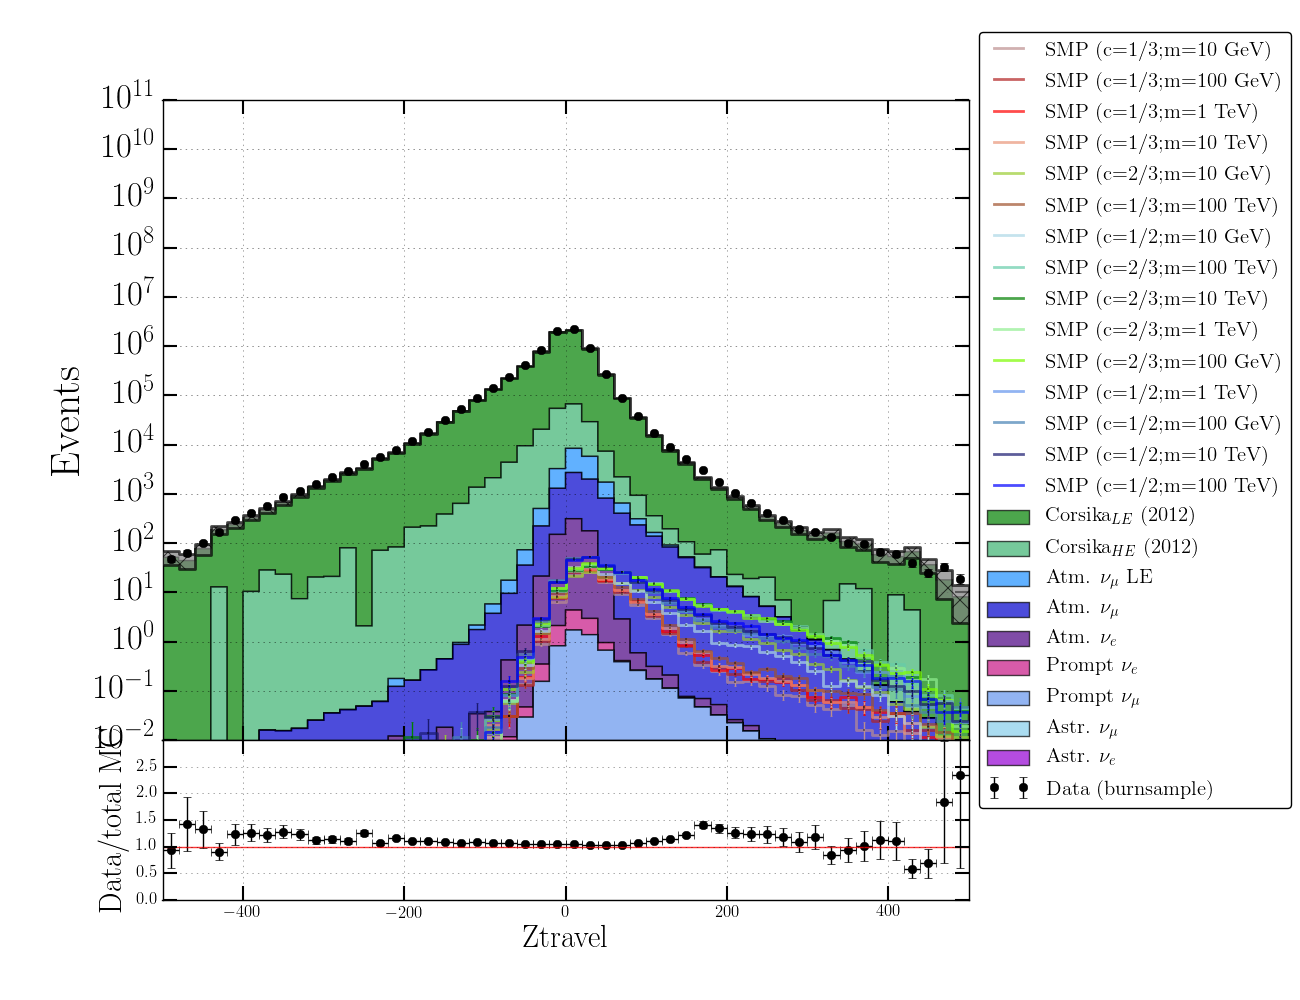
\includegraphics[width = 0.49\textwidth]{chapter8/img/1D_stack_ztravel.png}
\caption{Blub}
\label{fig:commonvariables1}
\end{figure}

\begin{figure}
\centering
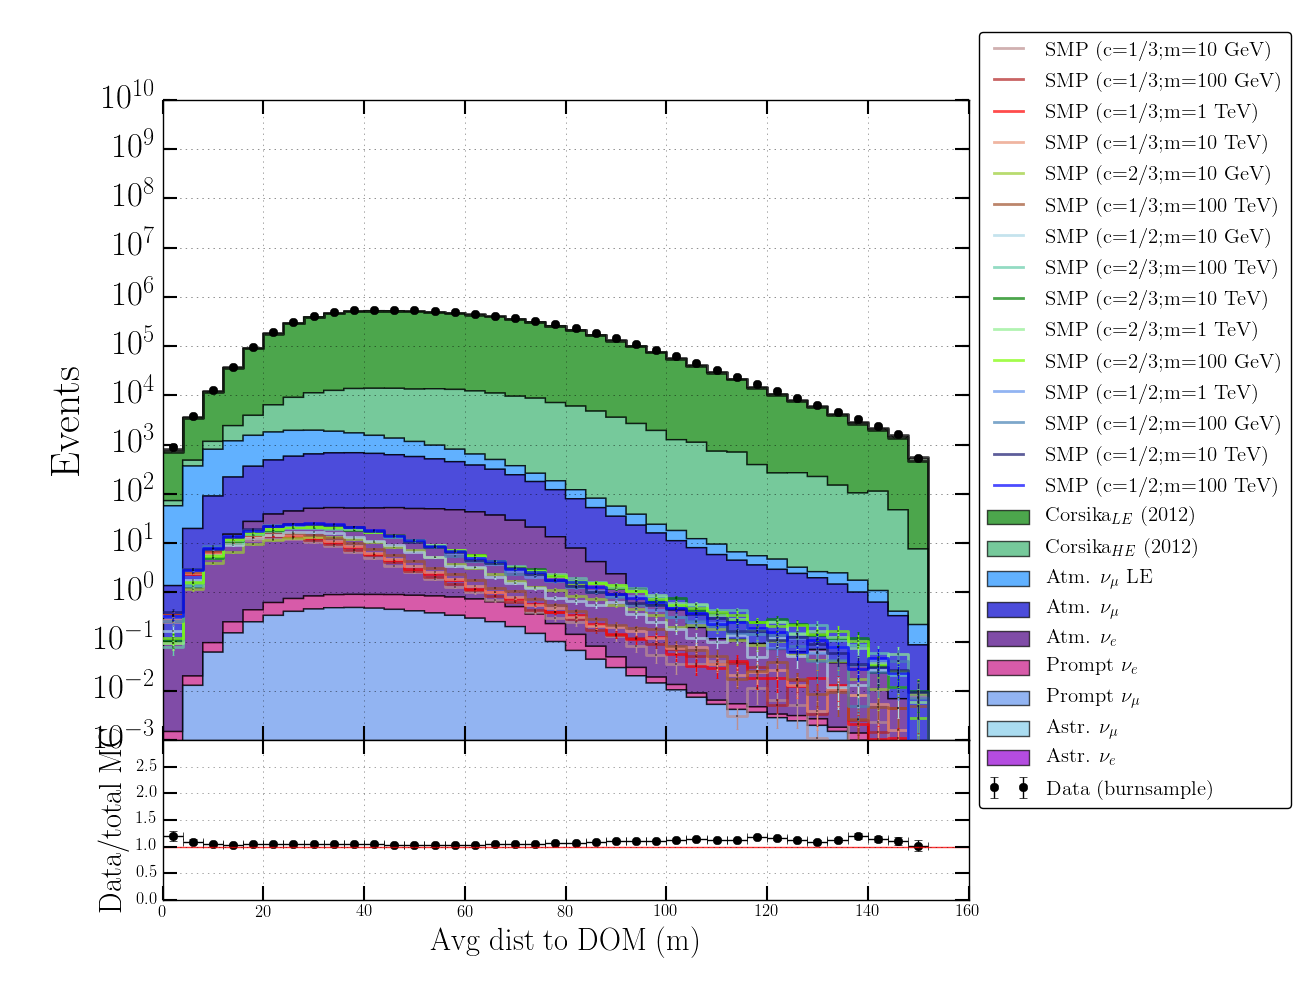
\includegraphics[width = 0.49\textwidth]{chapter8/img/1D_stack_avdistdom_150.png}
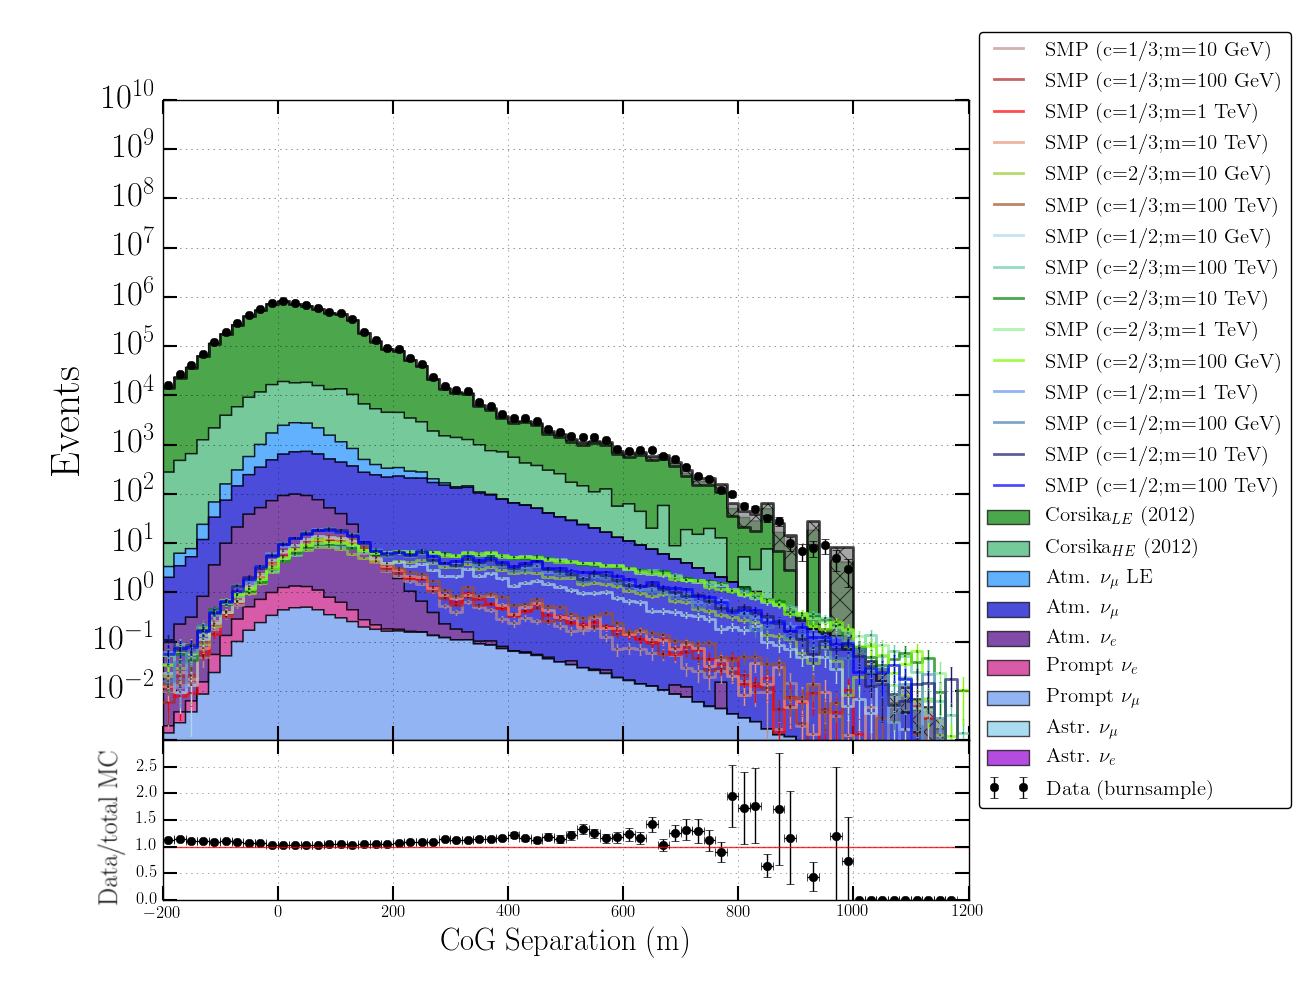
\includegraphics[width = 0.49\textwidth]{chapter8/img/1D_stack_trackseparation_150.png}
\caption{Blub}
\label{fig:commonvariables2}
\end{figure}

\begin{figure}
\centering
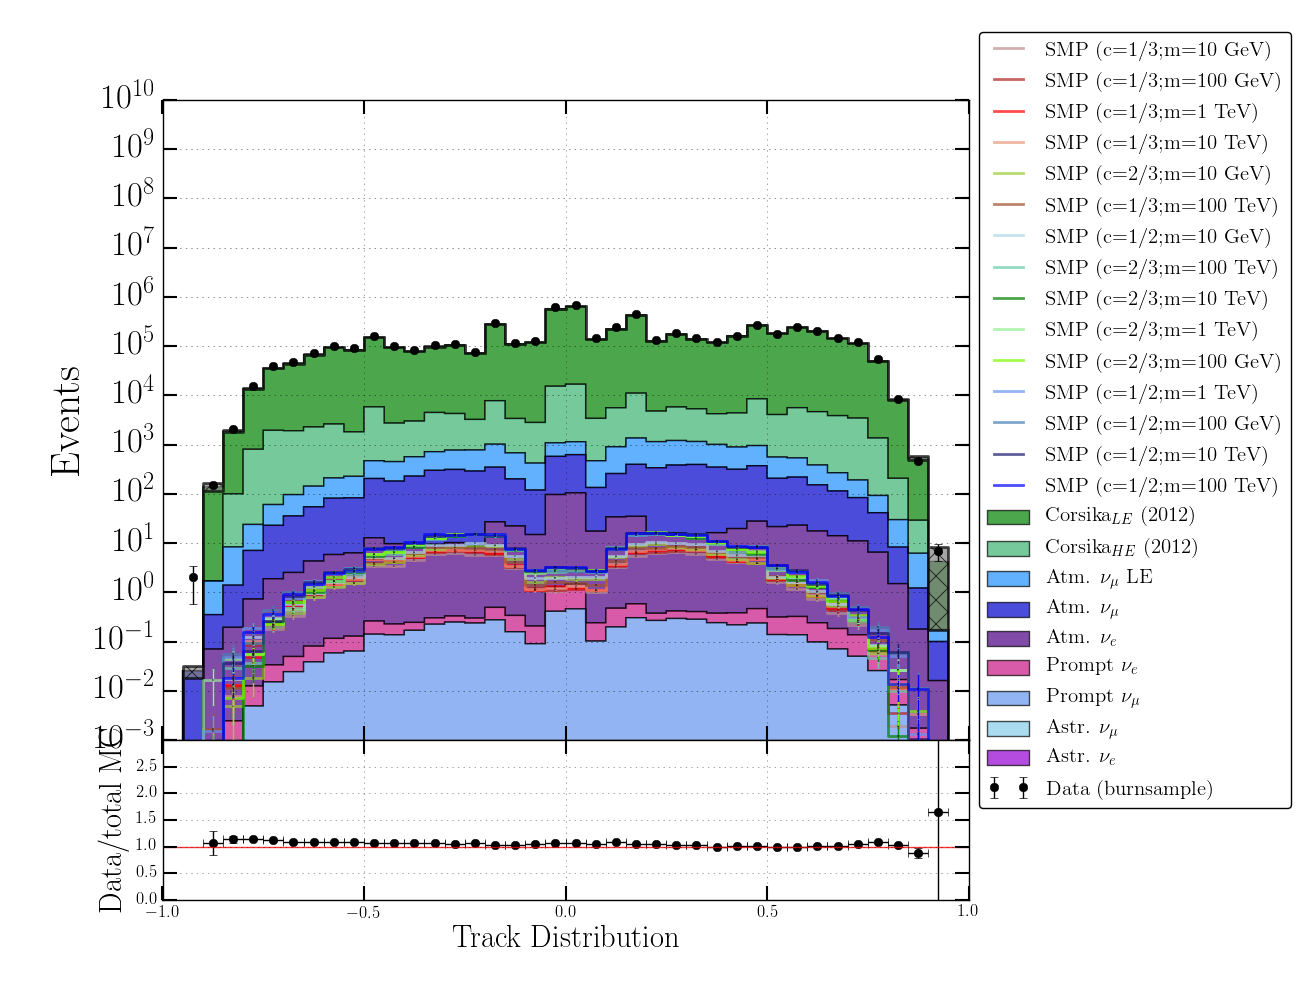
\includegraphics[width = 0.49\textwidth]{chapter8/img/1D_stack_trackdistribution_50.png}
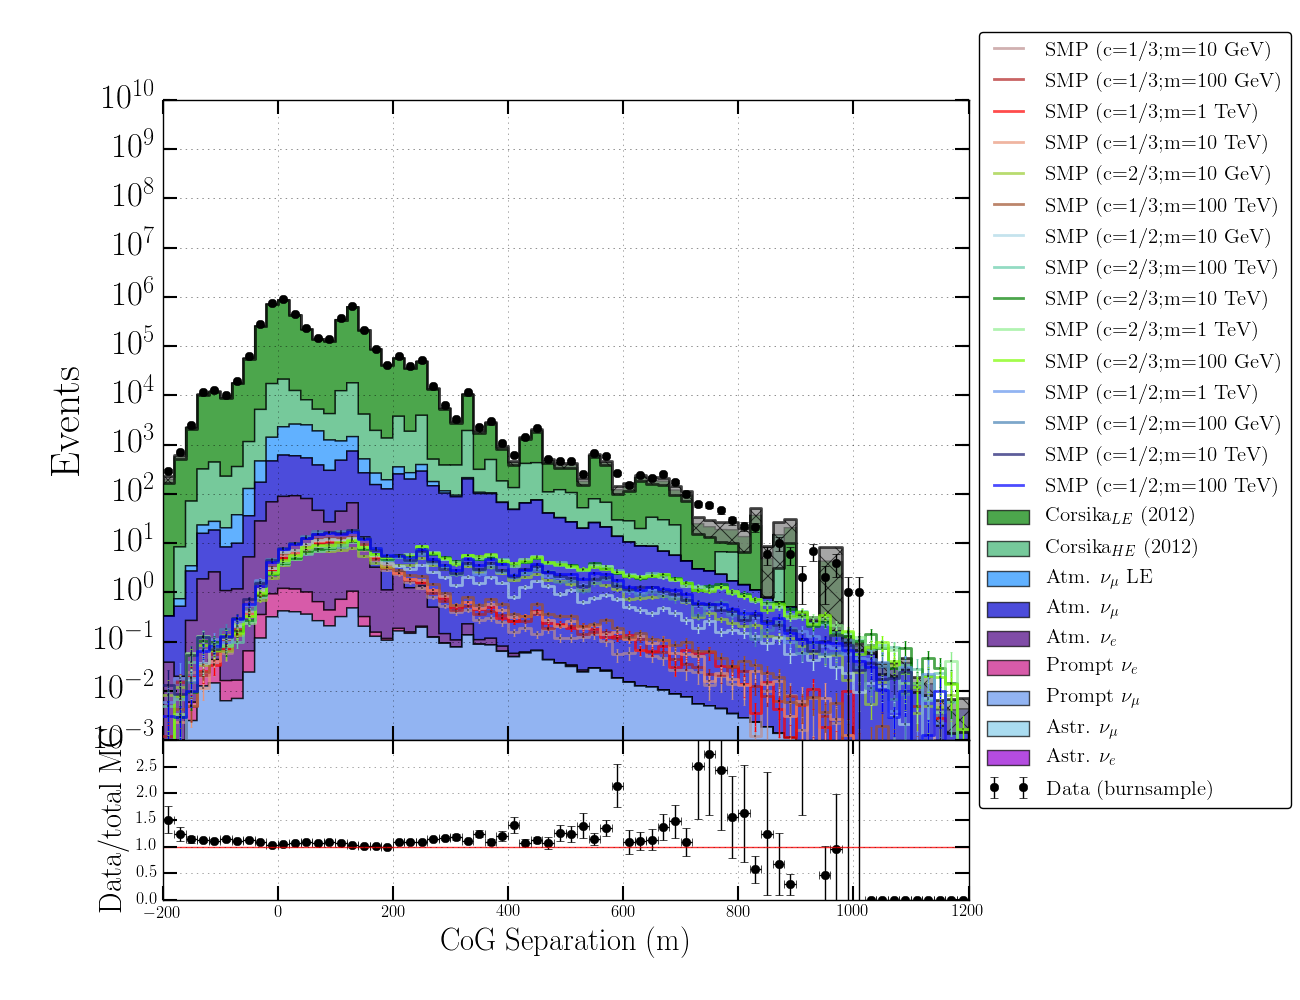
\includegraphics[width = 0.49\textwidth]{chapter8/img/1D_stack_trackseparation_50.png}
\caption{Blub}
\label{fig:commonvariables3}
\end{figure}

\begin{figure}
\centering
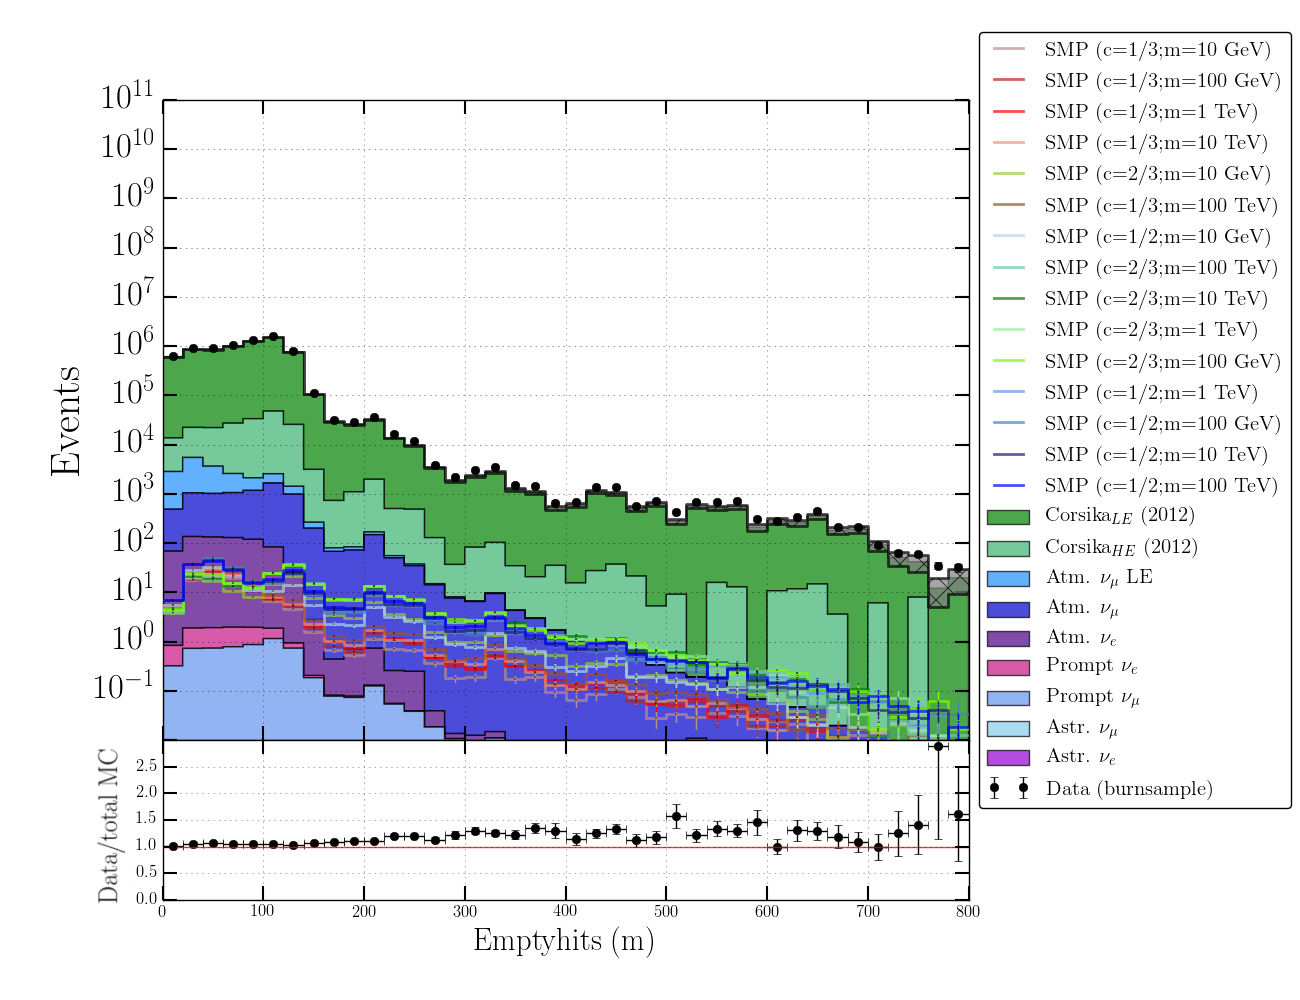
\includegraphics[width = 0.49\textwidth]{chapter8/img/1D_stack_emptyhits_100.png}
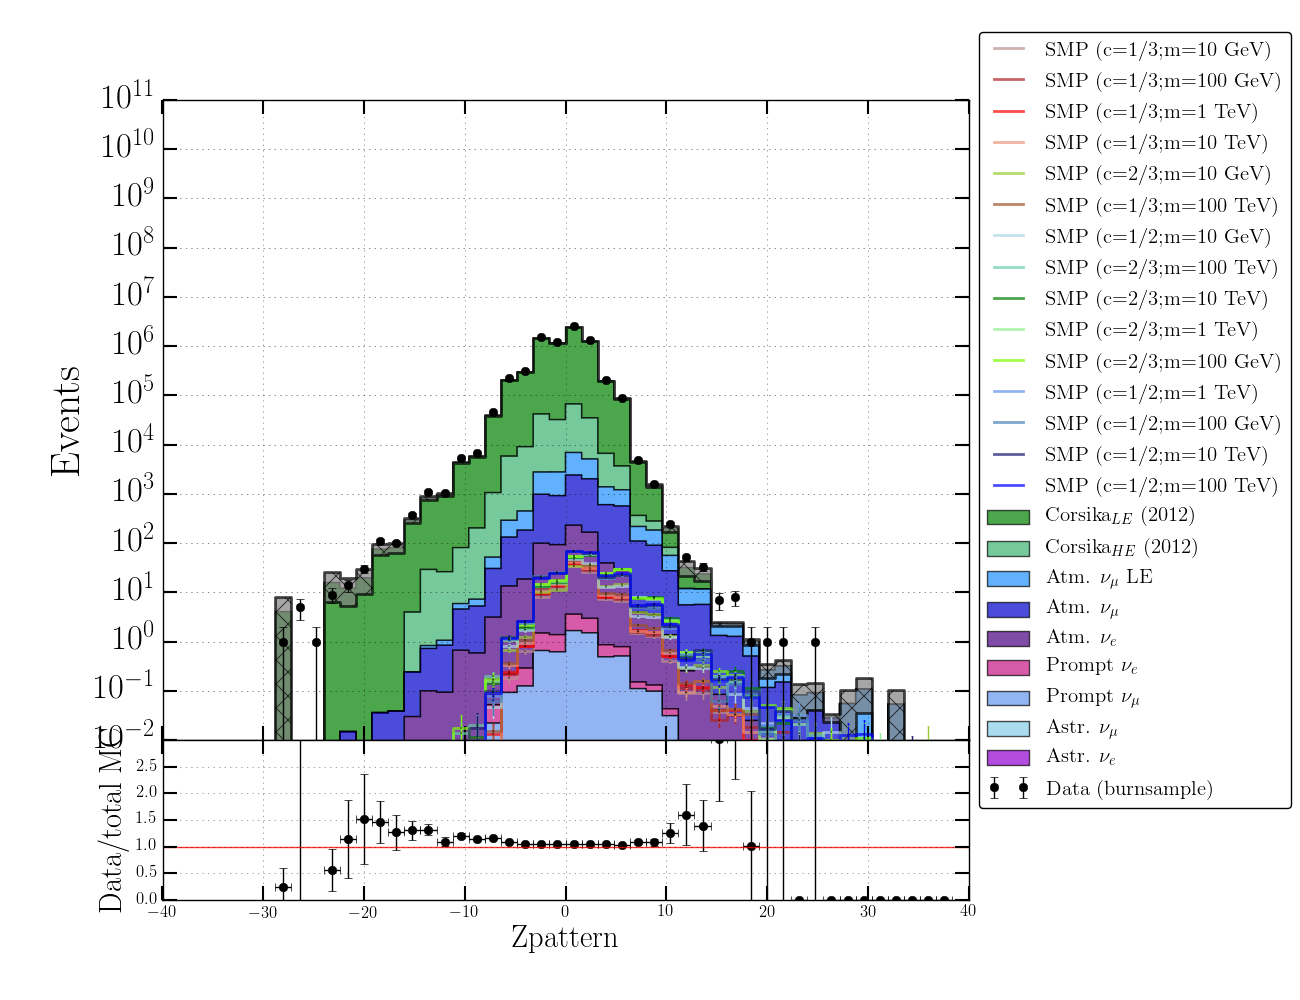
\includegraphics[width = 0.49\textwidth]{chapter8/img/1D_stack_zpattern.png}
\caption{Blub}
\label{fig:commonvariables4}
\end{figure}

Because DC and IC DOMs have different quantum efficiencies (see Section \ref{subsec:DC}), the pulses from DC and IC DOMs should not be mixed for an unambiguous definition. Therefore either only DC or IC pulses are used to compute these variables depending on if an event is \textit{IC dominated} or \textit{DC dominated}, where the former is set at $\frac{\# \textrm{DOMs}_\textrm{IC}}{\# \textrm{DOMs}_\textrm{DC}} >= 0.5$ and the latter otherwise.

\subsubsection{Millipede variables}
The \texttt{Millipede} toolkit was introduced in Section \ref{subsec:millipede}, where it was explained how the energy deposition could be estimated from the light seen by the individual DOMs. Constructing multiple variables from this toolkit was the master thesis subject of Stef Verpoest and can be found in Ref. \cite{steffthesis} for an elaborate explanation. The variables used in this analysis are explained below. Fig. \ref{fig:millipedeoutput} shows how the fit performed and can be helpful to explain the variables.

\begin{figure}[ht]
\centering
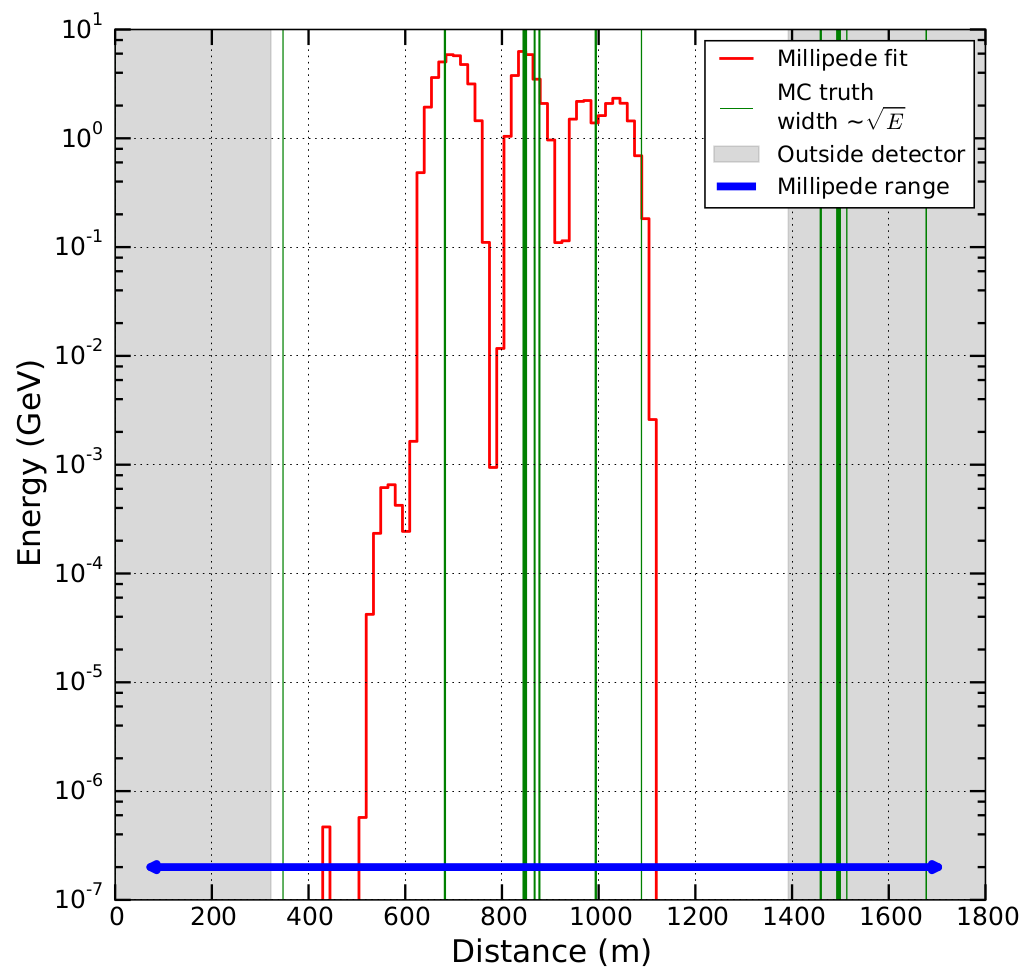
\includegraphics[width=0.6\textwidth]{chapter8/img/millipedeStef.png}
\caption{Output of a \texttt{Millipede} fit for an SMP with charge $\frac{1}{3}$ and mass 10 GeV. The x-axis shows the distance the particle traveled and starts after the first simulated energy loss event. The fit tries to estimate the energy of 15 m track segments. As a comparison, the true positions of energy deposits from the MC simulation are shown in green. Locations outside the detector are shaded in grey.}
\label{fig:millipedeoutput}
\end{figure}

\paragraph{Mean loss}
The most straightforward useage of the estimated mean energy loss rate is by taking the mean value and is referred to as \textit{Mean\_dEdX}. As can be seen from Fig. \ref{fig:allmillipedevar}, the distribution of SMPs peaks at lower values than known backgrounds as expected. Energy losses that are reconstructed to come from outside the detector are removed (hence the \textit{\_contained} in the figure). 

Due to the squared charge dependencies, an SMP of charge 1/3 is expected to have a relative energy loss difference to muons with a factor of 9, which is the case when comparing to muons from neutrino interactions. Atmospheric muons in this level are almost entirely the result of misreconstructions, corner clippers, etc. making a comparison not valid.
%Je wijkt af van de dEdX die je verwacht omdat je al voorgaande cuts hebt die kijken naar low E muons... 

\begin{figure}
\centering
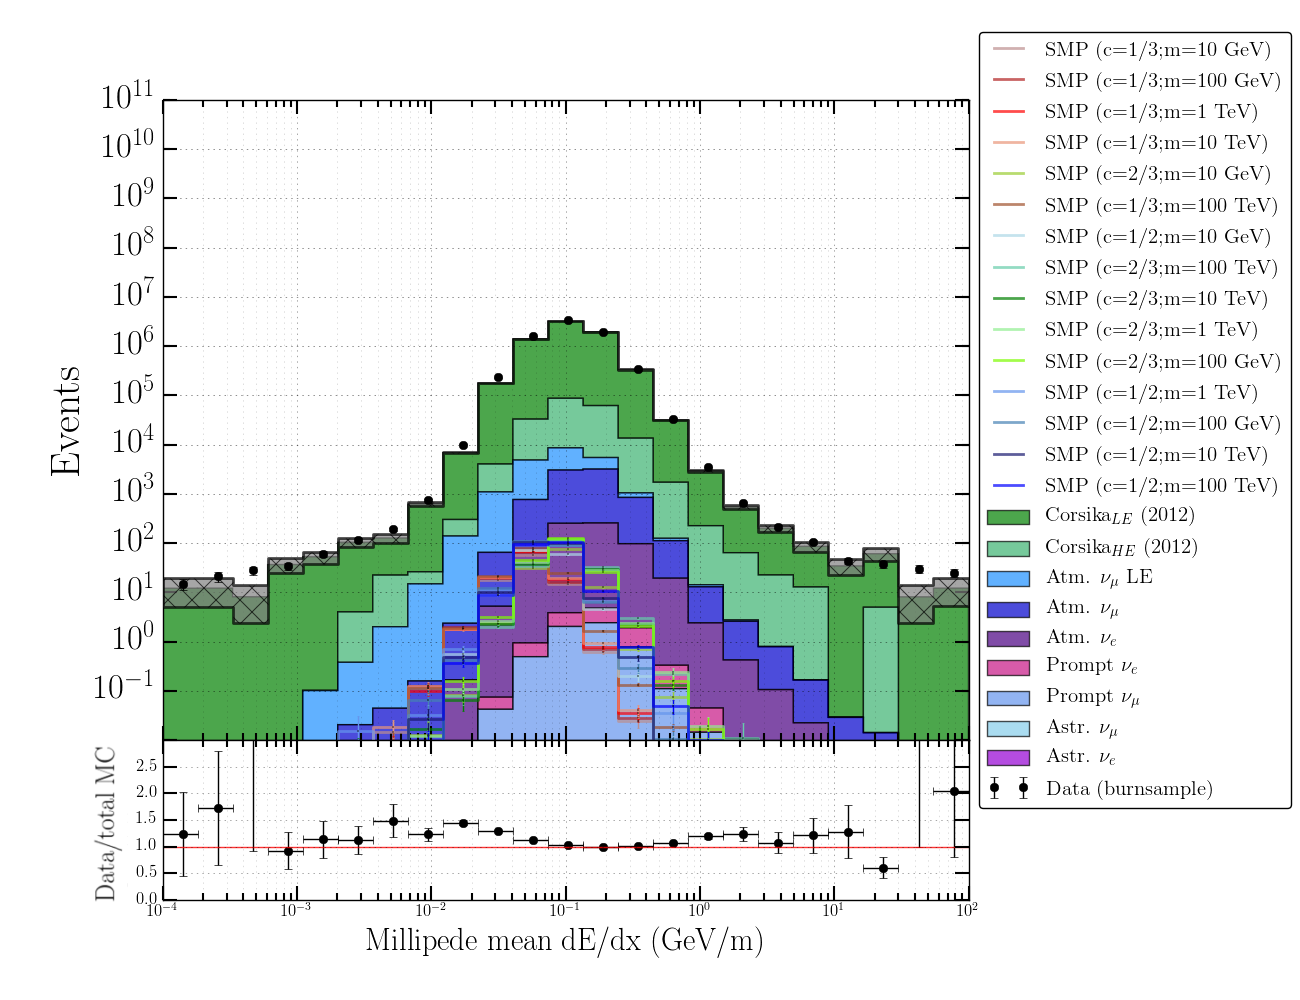
\includegraphics[width=0.49\textwidth]{chapter8/img/1D_stack_millipede_dedx_mean_nozeroes.png}
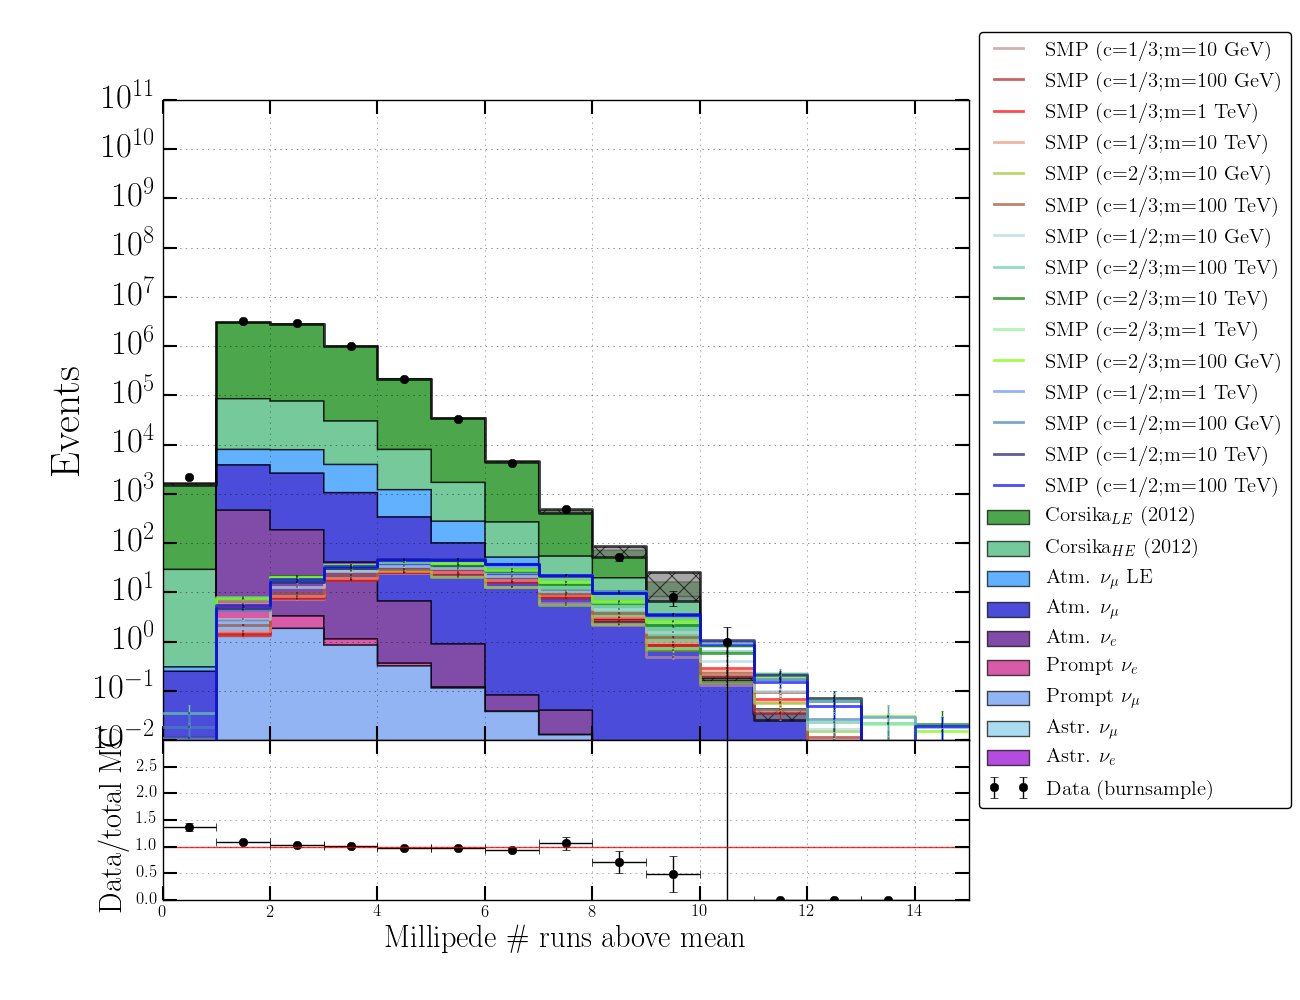
\includegraphics[width=0.49\textwidth]{chapter8/img/1D_stack_millipede_dedx_runsabovemean.png}
\caption{\textit{Left: }Distributions for the estimated mean energy loss from the \texttt{Millipede} toolkit. \textit{Right: }Distributions for the uniformity of the contained track.}
\label{fig:allmillipedevar1}
\end{figure}

\begin{figure}
\centering
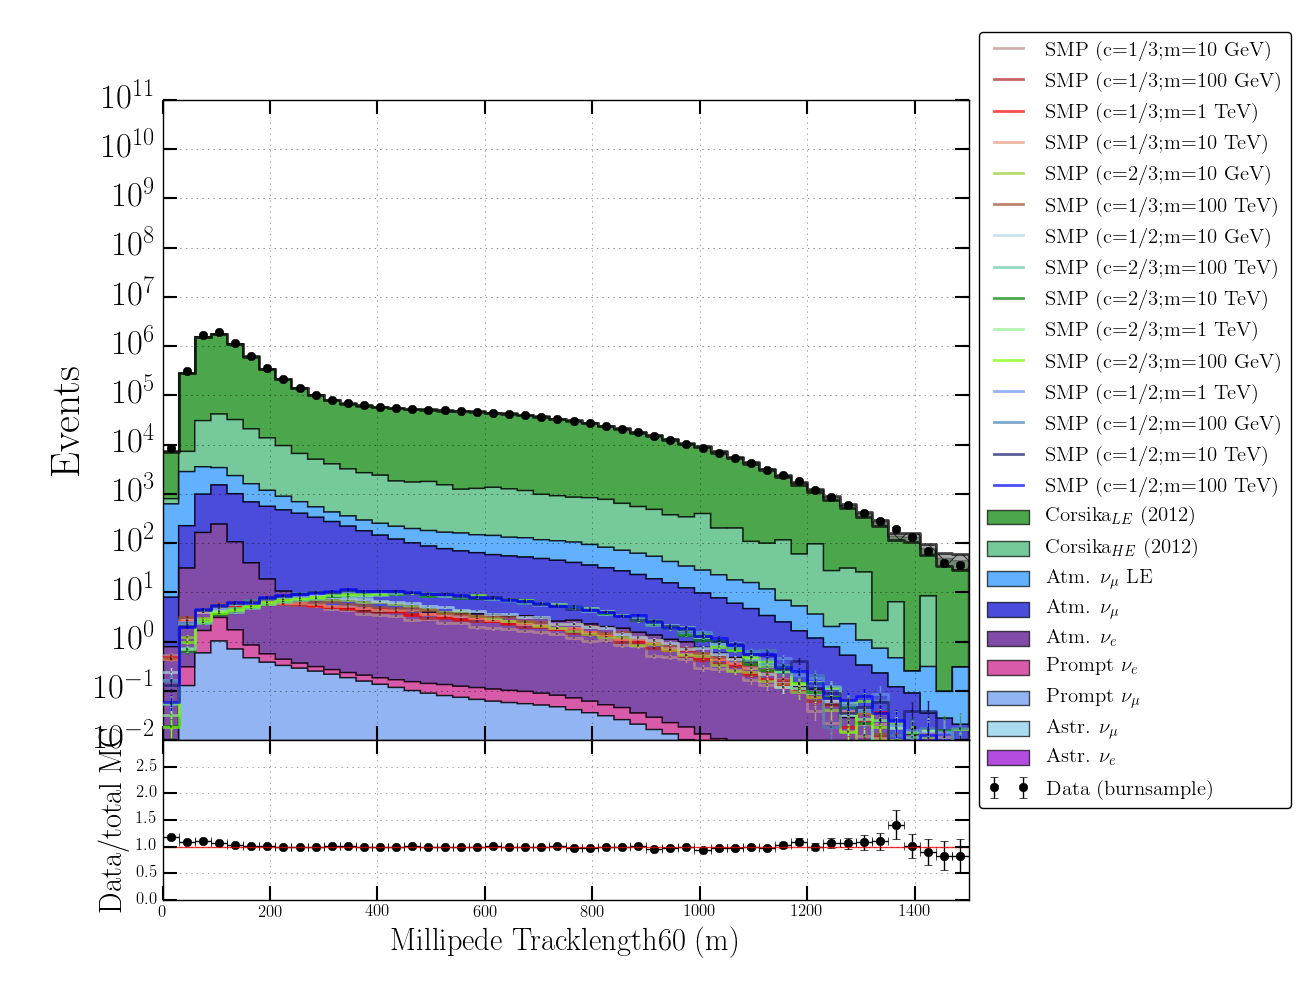
\includegraphics[width=0.49\textwidth]{chapter8/img/1D_stack_millipede_tracklength60.png}
\caption{Distributions for the track length of the particle where the \texttt{Millipede} segments are used instead of the DOM pulses.}
\label{fig:allmillipedevar2}
\end{figure}

\paragraph{Uniformity}
Once the mean is computed, it is possible to count the amount of times the energy distribution curve (red curve in Fig. \ref{fig:millipedeoutput}) to cross the mean value. This variable therefore parametrizes the uniformity of the track. The reasoning behind distriminating signal events from background is that most SMPs will have less uniform triggered hits due to the low amount of light that is produced. Particles therefore need to travel closer to a DOM to trigger a hit. In Fig. \ref{fig:allmillipedevar1} we can see that the background distributions peak at lower values than the signal, which also has a slower dropoff. 

\paragraph{Track length}
Because of the lower energy losses, the SMP particles are also expected to travel larger distances than muons, supporting the idea to contruct a variable that is sensitive to the distance traveled in the detector: a track length.

Since the tracks at this level are very dim, many segments from the \texttt{Millipede} output are reconstructed with zero energy. Therefore, it was chosen to use a certain part of the segments. The variables used here, \textit{TrackLength\_60}, used 60\% of the length where energy was deposited. It is the distance between the points where 20\% and 80\% of the deposited energy track segment. We expected to see larger tails in the distribution of Fig. \ref{fig:allmillipedevar2} in the signal compared to the background. Sub-optimal reconstructions result in bad millipede fits, giving a low and almost constant energy loss along the track. Additionally, coincident events that are not well separated also contribute to these events in the tail. However, most of the backgrounds events result into low values for this variable, still making it a powerful discriminative tool. 

\subsubsection{New variables}

\paragraph{Speedratio}
In addition, new variables were constructed. One was adopted from Jan K\"unnen's Earth WIMP analysis \cite{kunnenthesis}. By looking at the ``speed ratio'' of the first to second and first to third HLC hits, it was used to remove wrongfuly simulated detector noise, helping in data/MC disagreement. In this analysis, it showed to provide for a modest addition to discriminating variables\footnote{Data and MC seem to agree well, which is probably due to the newer and better simulations.}. The \textit{Speedratio} is defined as

\begin{equation}
\frac{v_{12}}{v_{13}} = \frac{d\left( \textrm{HLC}_1,\textrm{HLC}_2 \right)/\Delta t\left(\textrm{HLC}_1, \textrm{HLC}_2\right)}{d\left(\textrm{HLC}_1, \textrm{HLC}_3 \right)/\Delta t\left(\textrm{HLC}_1,\textrm{HLC}_3 \right)},
\end{equation}
where $d\left( \textrm{HLC}_i,\textrm{HLC}_j \right)$ is the distance between the DOMs that recorded the $i$th and $j$th HLC hits. $\Delta t\left(\textrm{HLC}_1, \textrm{HLC}_2\right)$ is the difference in time of the $i$th and $j$th HLC hits. This distribution is expected to peak at a value of 1, which is the expected result if one assumes that the photons originate from a particle traversing in a straight line and passes close to the DOMs. This is illustrated in Fig. \ref{fig:newvariables1}.

\begin{figure}
\centering
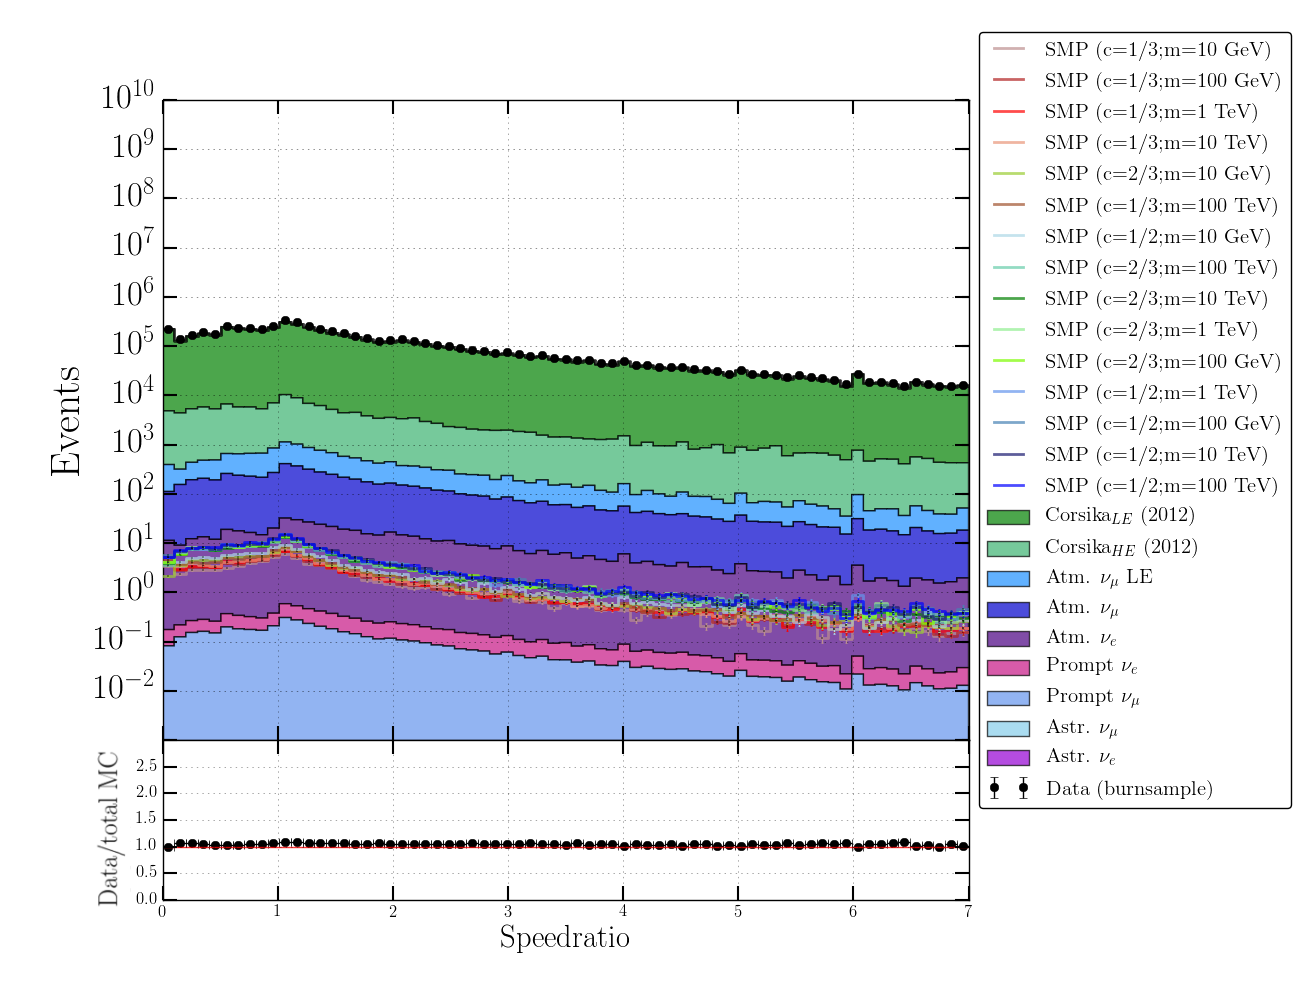
\includegraphics[width=0.49\textwidth]{chapter8/img/1D_stack_speedratio.png}
\caption{•}
\label{fig:newvariables1}
\end{figure}


\paragraph{NewLength}
Because DC and IC pulses should not be mixed, essential information is lost regarding the length of a track. Many signal events are DC dominated (see Section \ref{subsub:commonvariables}), making those track length variables not optimal. This is especially the case for events that have hits in both IC and DC and are far away from each other, which is not expected from low-energetic muons. These should, on average, produce more light than SMPs and not travel very far unless they have significant energies that would result in much higher light outputs. I have constructed new variables that use the MPE track reconstruction as a seed. First, the event is required to have 

\vspace{2mm}
\begin{itemize}
\item \#DC pulses $\geq$ 4,
\item \#IC pulses $\geq$ 2,
\end{itemize}
\vspace{2mm}
since otherwise the contribution of noise infiltration is too high. Additionaly,
pulses that lie within a cylinder with the seed track as the center are selected. The radius can be chosen, but is of the order of 50-150 meters. This radius is shown with a suffix after the variable (e.g. \_100), if the radius is infinite (all pulses are used), the suffix is ``\_all''. 

Then the first/last quartile in DC hits and the first/last half of the IC hits are determined. From these one can easily calculate the COG. To determine a length from four COGs, two have to be selected. The selection is based on the timing information on these COGs and given in the Table \ref{table:newlength}.\\

\begin{table}[h]
\caption{•}
\label{table:newlength}
\centering
\begin{tabular}{|
>{\columncolor[HTML]{F1A91E}}l |c|}
\hline
Timing & \cellcolor[HTML]{F1A91E}COG$_1$ \\ \hline
$\textrm{DC}_{f,q} < \textrm{IC}_{f,h}$ & DC$_{f,q}$ \\ \hline
$\textrm{DC}_{f,q} \geq \textrm{IC}_{f,h}$ & IC$_{f,h}$ \\ \hline
 & \cellcolor[HTML]{F1A91E}COG$_2$ \\ \hline
$\textrm{DC}_{l,q} > \textrm{IC}_{l,h}$ & DC$_{l,q}$ \\ \hline
$\textrm{DC}_{f,q} \leq \textrm{IC}_{f,h}$ & IC$_{l,h}$ \\ \hline
\end{tabular}
\end{table} 
 
\noindent All in all one can say that the NewLength variable is another attempt in defining the track length of the track in the detector. The suffix ``\_z'' is used for the variable that only uses the z-coordinate. Negative values occur when the timing of the two selected COGs is inverted when compared to the seed track (e.g. if the seed track is downgoing but the first CoG in time is located below the second COG) and most often occurs when the reconstruction was not optimal.\\

\noindent An illustration how the NewLength variable is constructed is shown in Fig. \ref{fig:newlength} and the distributions in Fig. \ref{fig:newvariables2}.

\begin{figure}
\centering
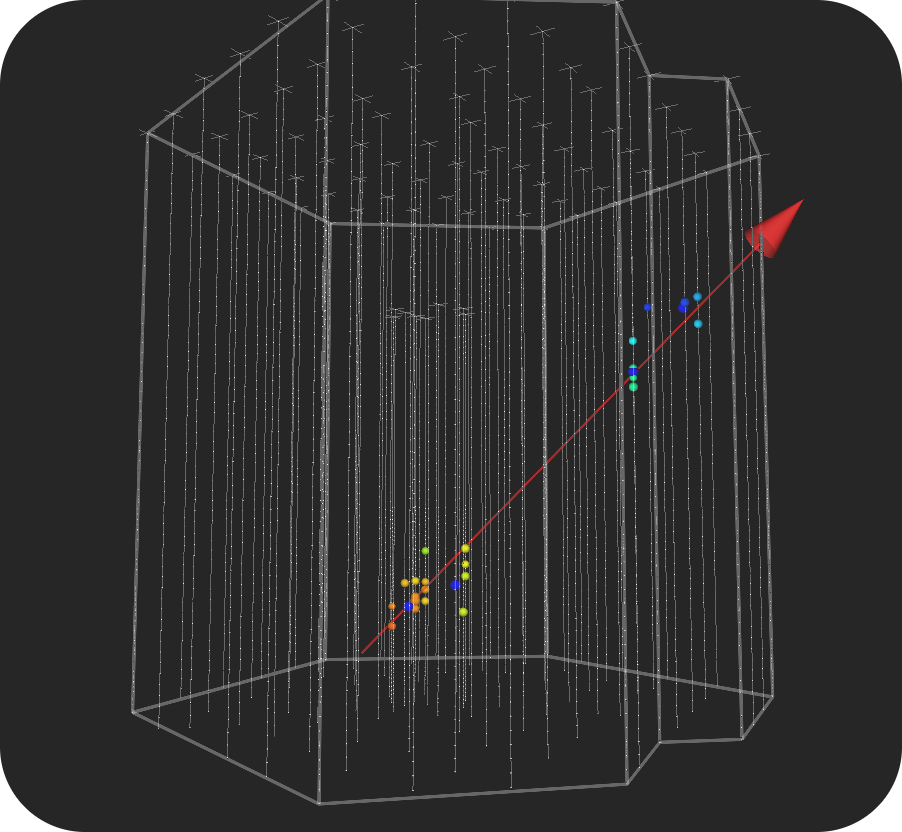
\includegraphics[width=0.6\textwidth]{chapter8/img/newlengthillustration.png}
\caption{The NewLength variable is constructed by selecting the first quartile/half of the COGs of DC/IC and computing the distance from the last quartile/half of the COGs of DC/IC. Out of the four, the first and last in pulse time are chosen to compute the distance.}
\label{fig:newlength}
\end{figure}
 

\begin{figure}
\centering
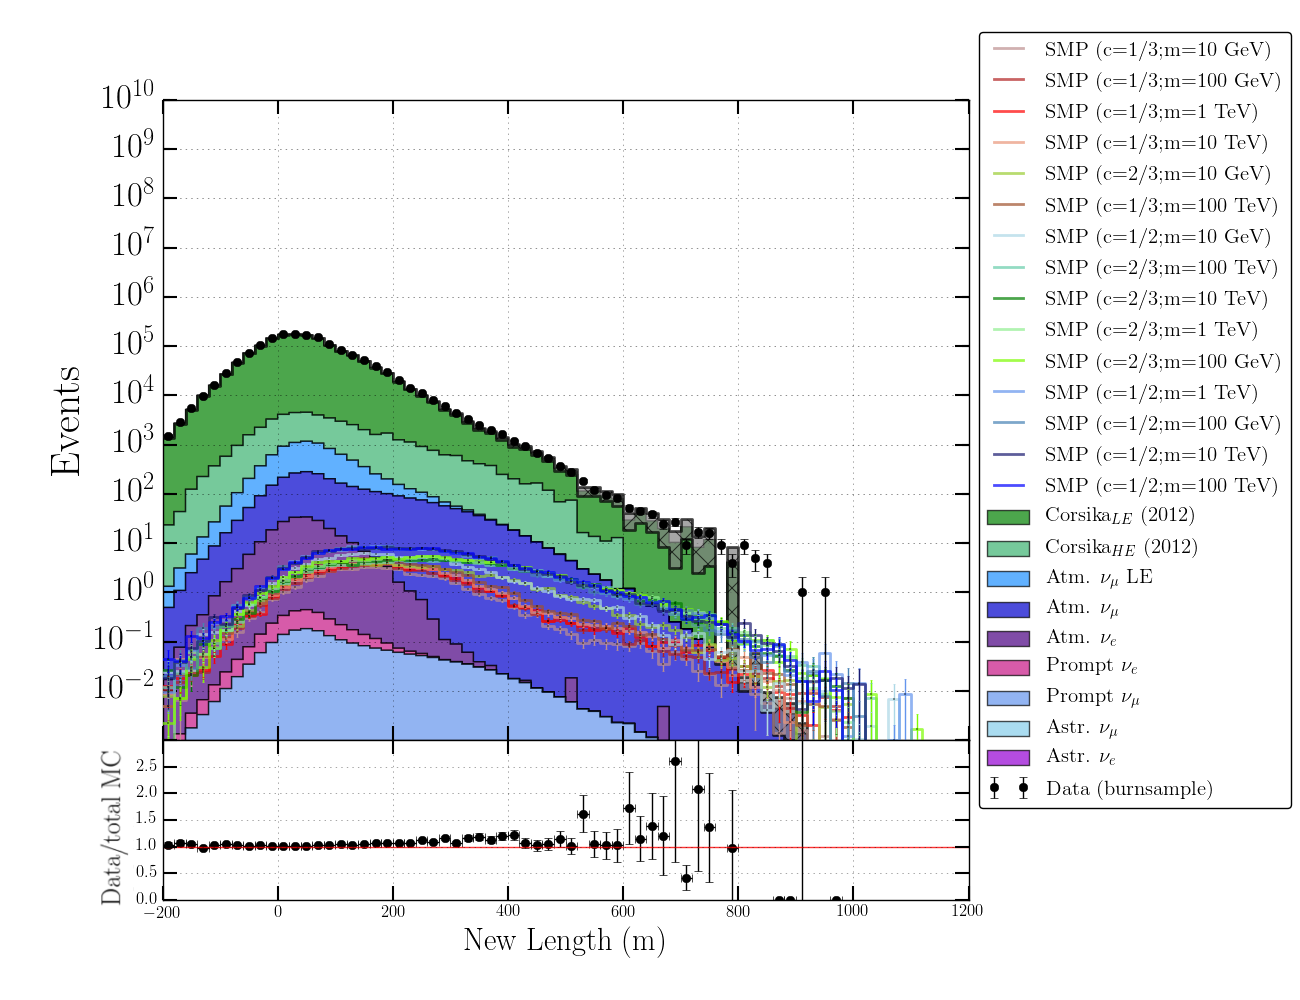
\includegraphics[width=0.49\textwidth]{chapter8/img/1D_stack_newlength_150.png}
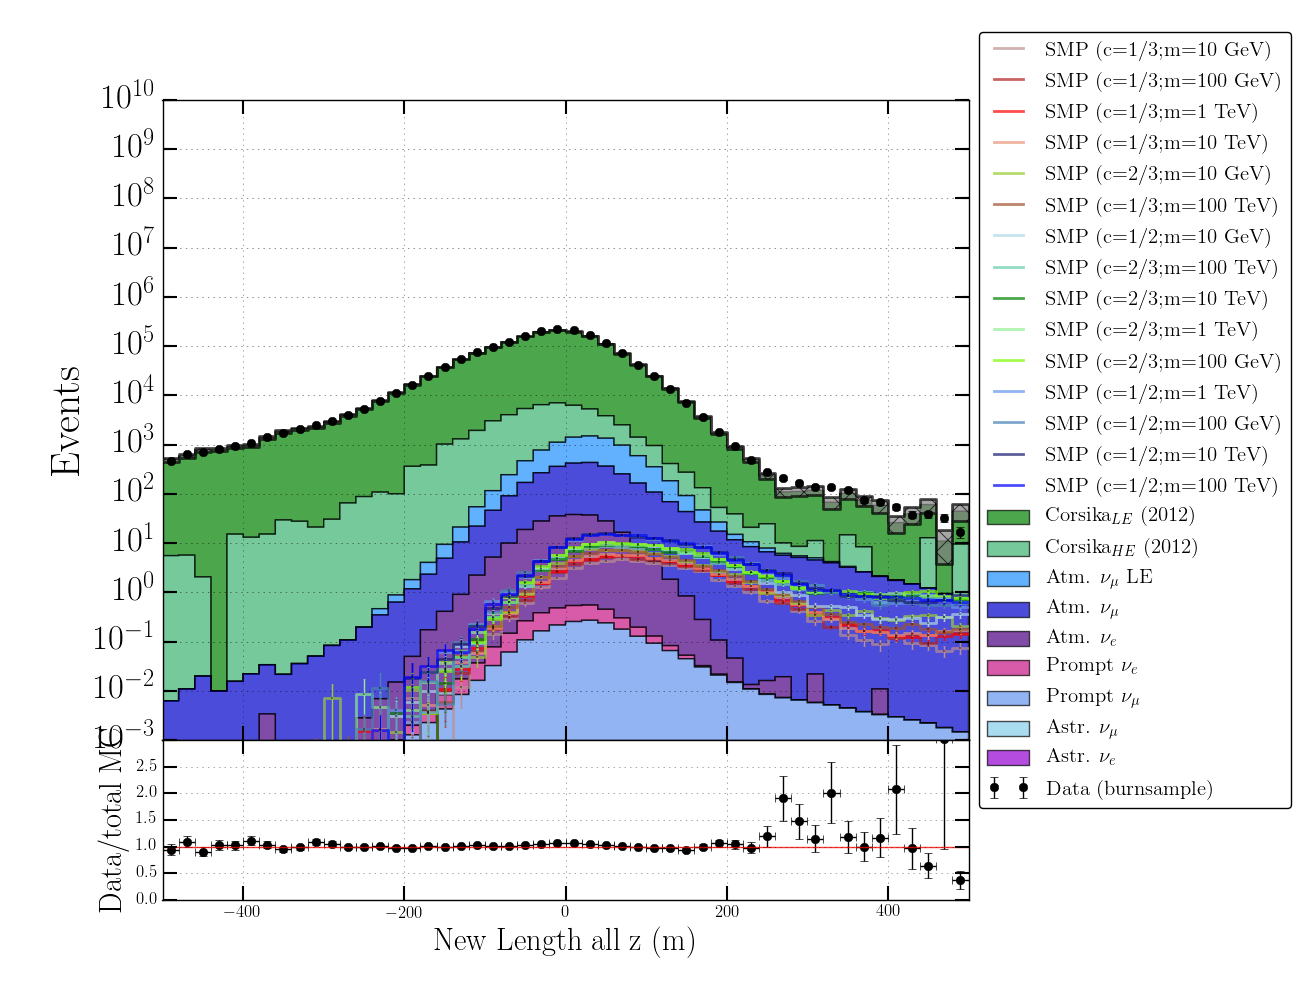
\includegraphics[width=0.49\textwidth]{chapter8/img/1D_stack_newlength_all_z.png}
\caption{•}
\label{fig:newvariables2}
\end{figure}

\begin{figure}
\centering
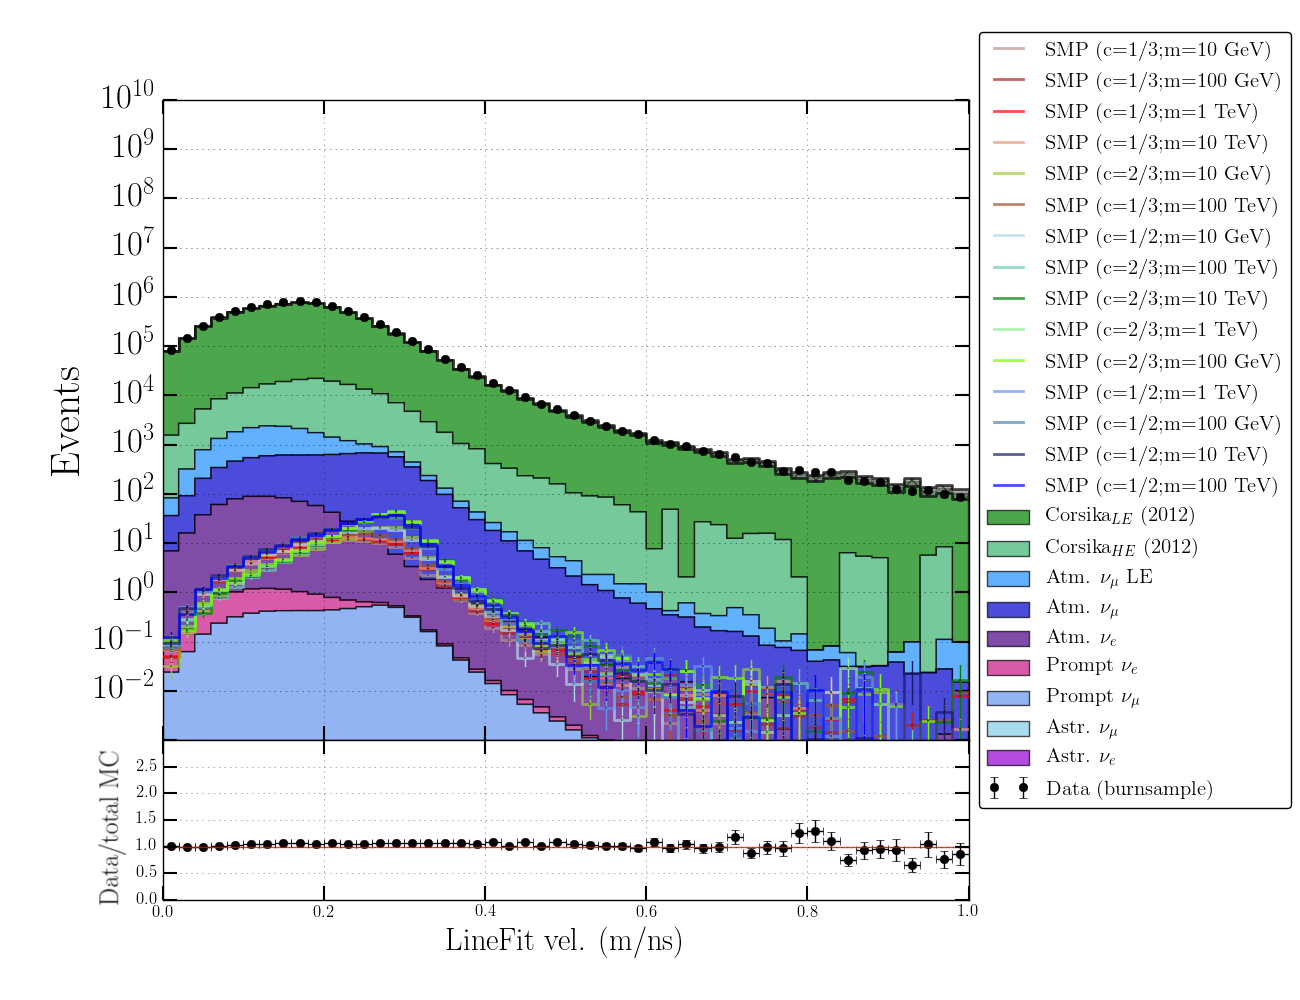
\includegraphics[width=0.49\textwidth]{chapter8/img/1D_stack_linefitvelocity}
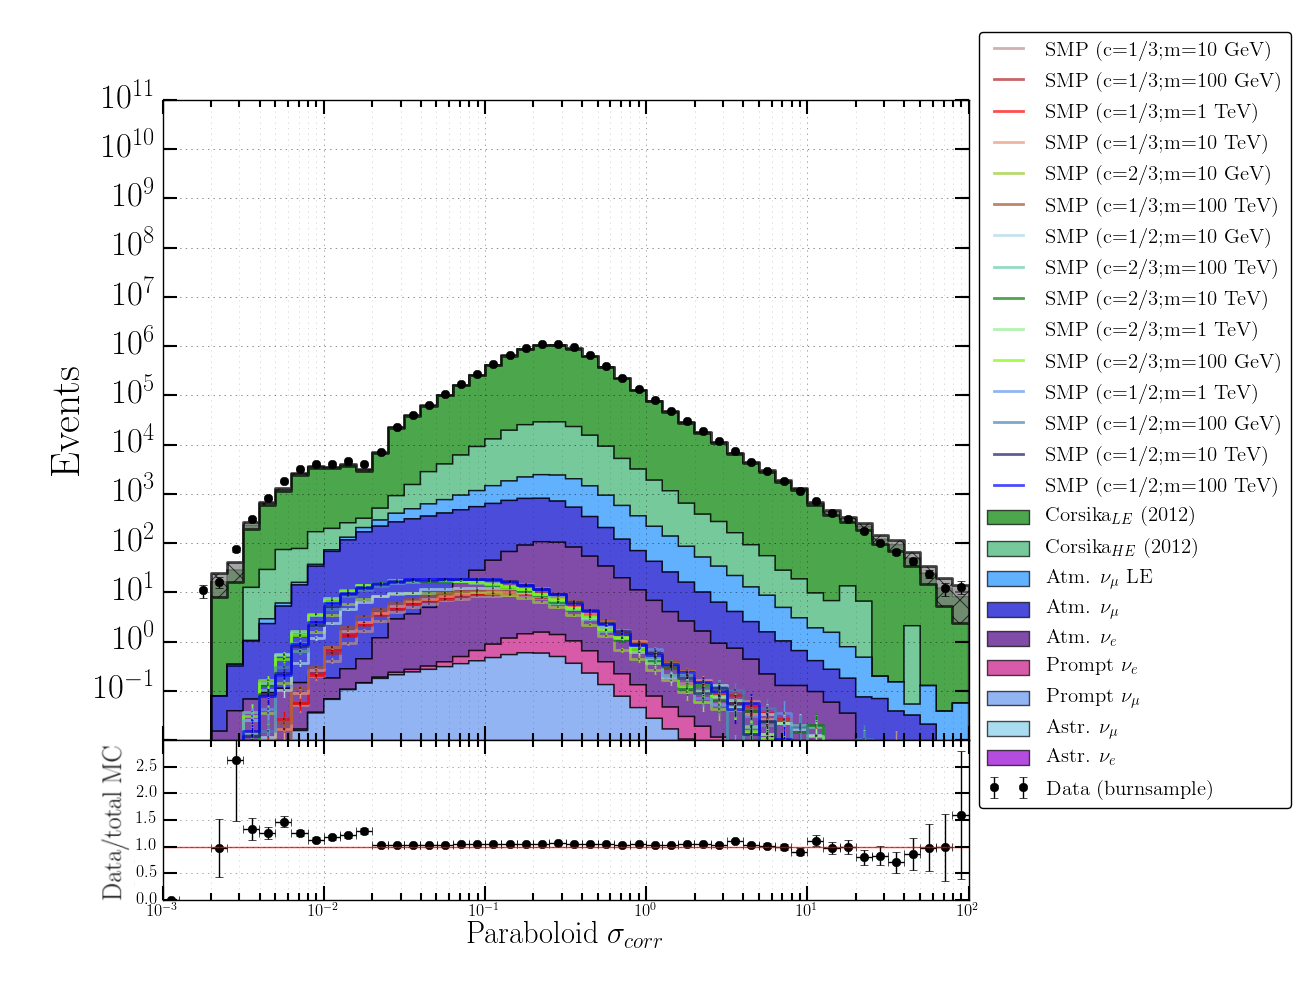
\includegraphics[width=0.49\textwidth]{chapter8/img/1D_stack_sigma_corr_paraboloid}
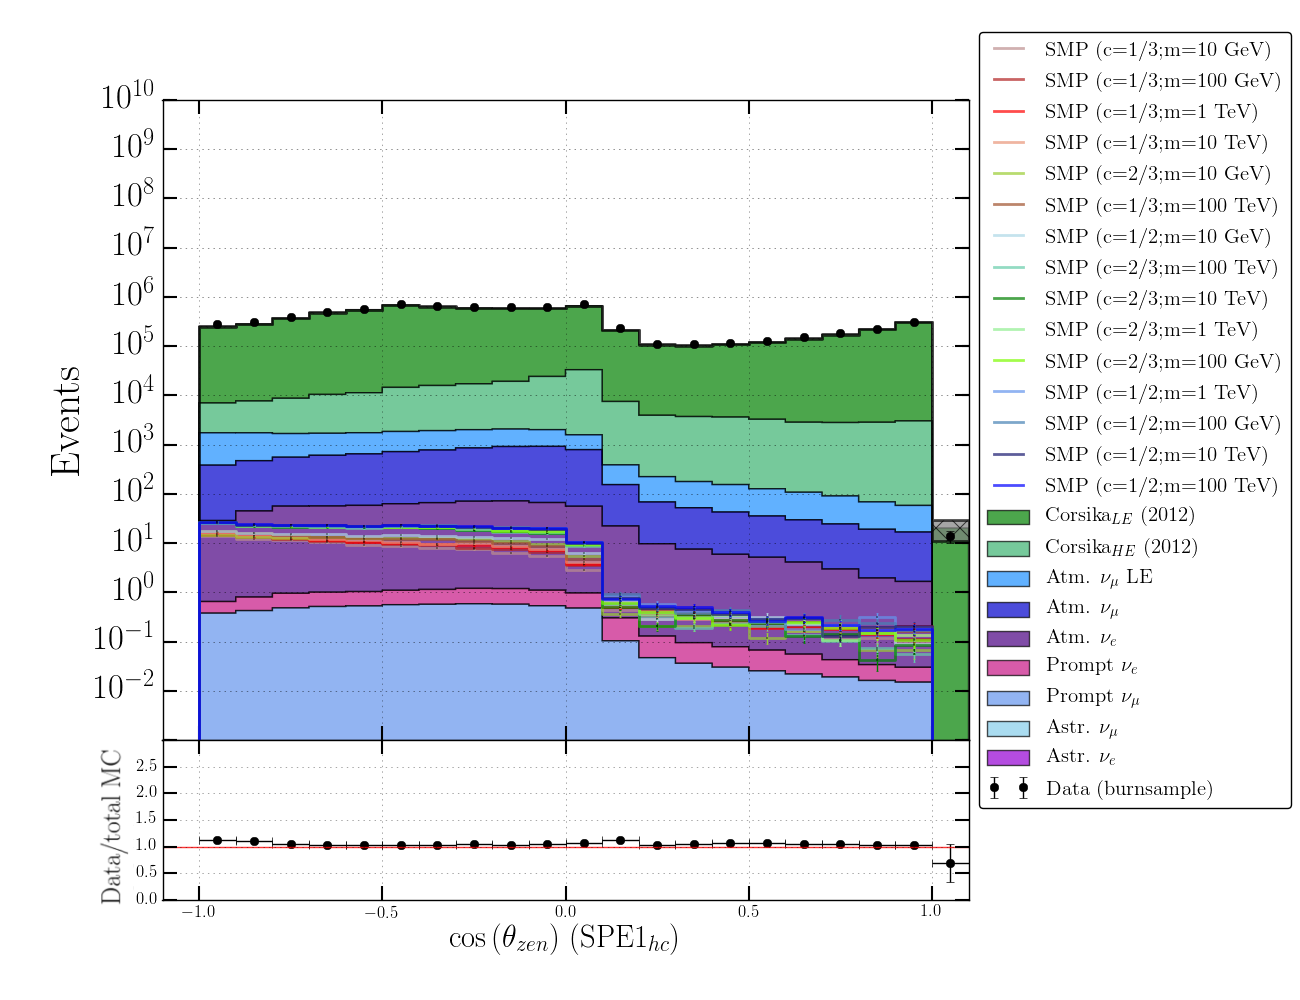
\includegraphics[width=0.49\textwidth]{chapter8/img/1D_stack_spefit1_hc_coszenith}
\caption{Blub}
\label{fig:remainingvariables}
\end{figure}

\subsection{Variable selection}
The variables that are used in the BDT in Level 5 were selected by using the mRMR technique explained in Section \ref{sec:mrmr}. The 17 most important variables were used in the BDT. Less variables meant a lower performance while more variables did not show to add additional power in the BDT performance and meant more computational power. An overview of these variables is shown in Tab. \ref{tab:mrmrimportance}.

\begin{table}[]
\footnotesize
\caption{My caption}
\label{tab:mrmrimportance}
\begin{tabular}{|l|r|c|c|}
\hline
\rowcolor[HTML]{F1A91E} 
Class & \multicolumn{1}{|c|}{Variable} & \begin{tabular}[c]{@{}c@{}}MRMR\\score\end{tabular} & \multicolumn{1}{l|}{\cellcolor[HTML]{F1A91E}Importance} \\ \hline
\multicolumn{1}{|c|}{\cellcolor[HTML]{F1A91E}} & ZMax & 2 & 0.109 \\ \cline{2-4} 
\multicolumn{1}{|c|}{\cellcolor[HTML]{F1A91E}} & ZTravel & 3 & 0.106 \\ \cline{2-4} 
\multicolumn{1}{|c|}{\cellcolor[HTML]{F1A91E}} & AvgDistToDom\_150 & 9 & 0.048 \\ \cline{2-4} 
\multicolumn{1}{|c|}{\cellcolor[HTML]{F1A91E}} & TrackSeparation\_150 & 10 & 0.043 \\ \cline{2-4} 
\multicolumn{1}{|c|}{\cellcolor[HTML]{F1A91E}} & TrackDistribution\_50 & 12 & 0.035 \\ \cline{2-4} 
\multicolumn{1}{|c|}{\cellcolor[HTML]{F1A91E}} & TrackSeparation\_50 & 13 & 0.034 \\ \cline{2-4} 
\multicolumn{1}{|c|}{\cellcolor[HTML]{F1A91E}} & EmptyHits\_100 & 16 & 0.027 \\ \cline{2-4} 
\multicolumn{1}{|c|}{\multirow{-8}{*}{\cellcolor[HTML]{F1A91E}Commonvariables}} & ZPattern & 17 & 0.016 \\ \hline
\cellcolor[HTML]{F1A91E} & RunsAboveMean & 4 & 0.105 \\ \cline{2-4} 
\cellcolor[HTML]{F1A91E} & Mean\_dEdX & 5 & 0.074 \\ \cline{2-4} 
\multirow{-3}{*}{\cellcolor[HTML]{F1A91E}Millipede} & TrackLength\_60 & 11 & 0.039 \\ \hline
\cellcolor[HTML]{F1A91E} & NewLength\_150 & 1 & 0.132 \\ \cline{2-4} 
\cellcolor[HTML]{F1A91E} & NewLength\_all\_z & 6 & 0.059 \\ \cline{2-4} 
\multirow{-3}{*}{\cellcolor[HTML]{F1A91E}New variables} & SpeedRatio & 14 & 0.033 \\ \hline
\cellcolor[HTML]{F1A91E} & LineFit\_Velocity & 7 & 0.055 \\ \cline{2-4} 
\cellcolor[HTML]{F1A91E} & $\sigma_{\textrm{para}}$ & 8 & 0.051 \\ \cline{2-4} 
\multirow{-3}{*}{\cellcolor[HTML]{F1A91E}Other variables} & $\cos(\theta)_{\textrm{SPE}}$ & 15 & 0.033 \\ \hline
\end{tabular}
\begin{tabular}{|c|r|}
\hline
\rowcolor[HTML]{F1A91E} 
\begin{tabular}[c]{@{}c@{}}MRMR\\score\end{tabular}& Variable \\ \hline
\cellcolor[HTML]{F1A91E} 1 & NewLength\_150 \\ \hline
\cellcolor[HTML]{F1A91E} 2 & ZMax \\ \hline
\cellcolor[HTML]{F1A91E} 3 & ZTravel \\ \hline
\cellcolor[HTML]{F1A91E} 4 & RunsAboveMean \\ \hline
\cellcolor[HTML]{F1A91E} 5 & Mean\_dEdX \\ \hline
\cellcolor[HTML]{F1A91E} 6 & NewLength\_all\_z \\ \hline
\cellcolor[HTML]{F1A91E} 7 & LineFit\_Velocity \\ \hline
\cellcolor[HTML]{F1A91E} 8 & $\sigma_\textrm{para}$ \\ \hline
\cellcolor[HTML]{F1A91E} 9 & AvgDistToDom\_150 \\ \hline
\cellcolor[HTML]{F1A91E} 10 & TrackSeparation\_150 \\ \hline
\cellcolor[HTML]{F1A91E} 11 & TrackLength\_60 \\ \hline
\cellcolor[HTML]{F1A91E} 12 & TrackDistribution\_50 \\ \hline
\cellcolor[HTML]{F1A91E} 13 & TrackSeparation\_50 \\ \hline
\cellcolor[HTML]{F1A91E} 14 & SpeedRatio \\ \hline
\cellcolor[HTML]{F1A91E} 15 & $\cos(\theta)_\textrm{SPE}$ \\ \hline
\cellcolor[HTML]{F1A91E} 16 & EmptyHits\_100 \\ \hline
\cellcolor[HTML]{F1A91E} 17 & ZPattern \\ \hline
\end{tabular}
\end{table}

\section{Level 5}
The last part of the analysis makes use of the variables that were constructed and the 17 that were estimated from the mRMR technique as the most powerful. First, the result from a single BDT is shown. Due to the lack of statistics in the final selection, the pullvalidation method was used for a limit computation.

\subsection{BDT result}
The parameters that were used for BDT training (see Section \ref{sec:BDT}) are:
\vspace{2mm}
\begin{itemize}
\item Maximal depth: 2 (Fig. \ref{fig:bdt})
\item Boosting $\beta$: 0.8 (Eq. \ref{eq:boostfactor})
\item Number of trees: 400 (Section \ref{subsec:boosting})
\item Pruning factor: 35 (Section \ref{subsub:pruning})
\end{itemize}
\vspace{2mm}
\noindent Training is done on 10\% of the available burnsample as it showed to have a much better performance as opposed to training on background simulation due to the limited amount of CORSIKA simulation available. The other 90\% of the burnsample is used for testing and is shown in the following plots. Testing on the MC datasets is also shown for the sake of completeness. Contribution of possible signal events, if they exist, in the data are minimal. Together with the very good data/MC agreement that is seen in the variables used, the training on data is a valid choice.

Also, it was chosen to select a (large) subsample of the signal to train the BDT to give the best possible results. One can see in the variable distributions in Figs. \ref{fig:commonvariables4} and \ref{fig:newvariables2} that there are minimal contributions of events with negative ZTravel and/or negative NewLength values. Upgoing tracks should give positive values both and are therefore removed from the signal sample that is used to train the BDT\footnote{Of course, the final signal rate is computed from the full signal sample.}.\\

\noindent The result of one BDT can be seen in Fig. \ref{fig:singlebdtrate} and we can draw several conclusions:
\vspace{2mm}
\begin{itemize}
\item Data and MC show a very good agreement.
\item The rate in background events is reduced with 4 to 5 orders of magnitude at the a BDT score around 0.25.
\item At highere BDT scores, muons from low energetic muon neutrinos become a much more significant part of the total background than muons from air showers.
\item The signal used to train the BDT is more concentrated at higher scores, as expected. The total signal sample and the subset used for training overlap at scores higher than 0.1.
\item At the highest scores, where the signal dominates, it is clear that there is a lack of statistics in both CORSIKA simulations as the burn sample.
\end{itemize}
\vspace{2mm}

\begin{figure}
\centering
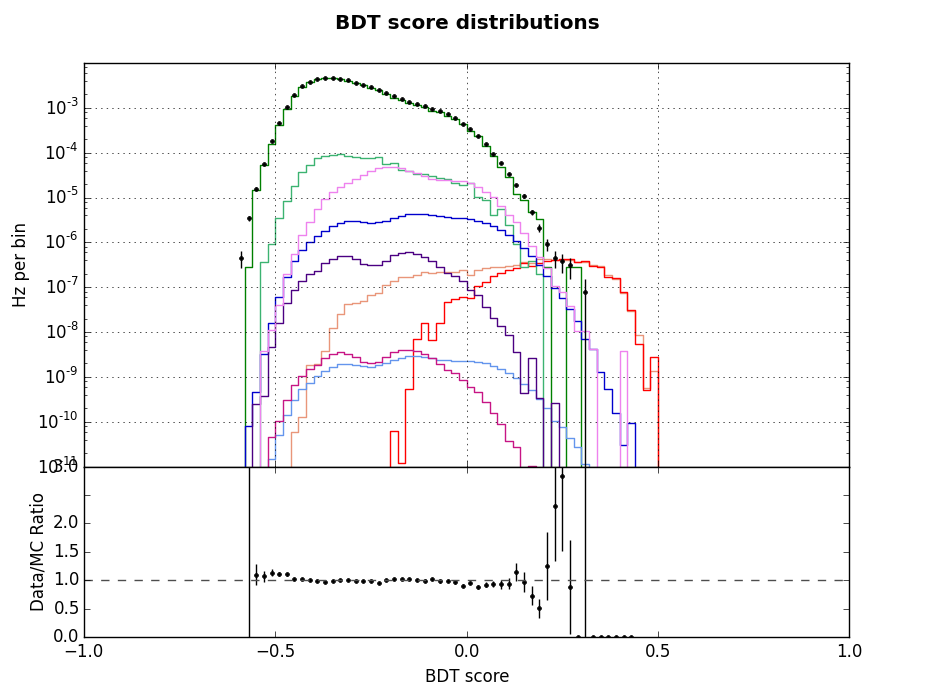
\includegraphics[width = 0.7\textwidth]{chapter8/img/dist_vs_bdt_result2_signal_m_100_charge1ovr2.png}
\caption{Blub}
\label{fig:singlebdtrate}
\end{figure}



\url{https://arxiv.org/pdf/physics/0312102v1.pdf}\\
\url{https://arxiv.org/pdf/1310.1284.pdf}

Ook ergens een tabel maken met info over je data runs. Duidelijk maken wat de livetime is bv en ook zeggen van wanneer to wanneer een bepaalde run liep (2011: mei 2011- mei 2012)

Klaus zijn paper? \url{https://arxiv.org/abs/1806.05696}


\section{Pull validation}
\section{Systematic Uncertainties}

\section{Results}